\documentclass[12pt,oneside,a4paper]{book}

% spis treści z semianarium
% 1 Wprowadzenie
% - cel i zakres pracy
% - podział pracy
% - założenia projektowe
% - analiza literatury
% 2 Budowa urządzenia / systemu / Opis oprogramowania / Teoria / Użyte Narzędzia
% 3 Implementacja / Optrogramowanie
% - zad. 1
% - zad. 2
% - zadania: poszczególne elementy projektu
% 4 Weryfikacja / Testy / Wyniki pomiarów / Analiza porównawcza wedłóg założeń
% 5 Podsumowanie (Nie pisać że to wnioski!) i Propozycje dalszego rozwoju / uwagi koncowe
% 6 Załączniki 

% Prezentacja do obrony pracy inżynierskiej - wspólnie - 10-15 minut, można trochę przedłużyć


\usepackage{polski}
\usepackage[utf8]{inputenc}
\usepackage{lmodern}
\usepackage{indentfirst}
\usepackage{microtype}
\usepackage{fancyhdr}
\usepackage{pstricks,graphicx}
\usepackage{amssymb}
\usepackage{theorem}
\usepackage{geometry}
\usepackage{amsmath}
\usepackage[hidelinks]{hyperref}
\usepackage{tabularx}
\usepackage{float}
\usepackage{import}

\import{.}{code_highlights.tex}

\DisableLigatures{encoding = *, family = * }

\def\bibname{Literatura}

\newcommand{\outputTxt}[1]{
    % \begin{shbox}[H]
    %     \centering
        % \textbf{Output:} \\
        \lstinputlisting{#1}
    % \end{shbox}
}

 
\theoremstyle{break}
\theorembodyfont{\it}
\newtheorem{twr}{Twierdzenie}[chapter]
\newtheorem{lem}{Lemat}[chapter]
\theorembodyfont{\rm}
\newtheorem{defi}{Definicja}[chapter]
\newtheorem{wni}{Wniosek}[chapter]
\newtheorem{prz}{Przykład}[chapter]
\newenvironment{dowod}{\par\vspace{0.1cm}\par{ \sc Dowód.}}{\hfill $\blacksquare$\par\vspace{0.4cm}\par}

\newgeometry{tmargin=2.5cm, bmargin=2.5cm, headheight=14.5pt, inner=3cm, outer=2.5cm} 

\hypersetup{
    colorlinks,
    citecolor=black,
    filecolor=black,
    linkcolor=black,
    urlcolor=black
}

\linespread{1.1}

\pagestyle{fancy} 

\graphicspath{{images/}}

\fancyhead[C]{} 
\fancyfoot[C]{\thepage}
\fancyhead[L]{\scriptsize\leftmark}
\fancyhead[R]{\scriptsize\rightmark}

\renewcommand{\chaptermark}[1]{
\markboth{\MakeUppercase{
\chaptername}\ \thechapter.
\ #1}{}}

\renewcommand{\sectionmark}[1]{\markright{\thesection.\ #1}}

\newcommand{\university}{Politechnika Poznańska}
\newcommand{\department}{Wydział Automatyki, Robotyki i Elektrotechniki}
\newcommand{\topic}{Bezprzewodowa sieć kontrolno-pomiarowa}
\newcommand{\authors}{Ryszard Napierała, Dawid Dziedzic}

\begin{document}
\thispagestyle{empty}
\begin{center}
    {\sc \Large \university}
    \par\vspace{0.2cm}\par
    {\large \department}
\end{center}
\vspace{1cm}
\begin{center}
    \includegraphics{warie_logo.png}
\end{center}
\begin{center}
    {\large Praca inżynierska dyplomowa}
    \par\vspace{0.2cm}\par
    {\LARGE \topic}
\end{center}
\begin{center}
    \authors, \\
    kierunek: Automatyka i robotyka
\end{center}
\par\vspace{3cm}\par
\begin{flushright}
    Promotor:\\
    dr inż. Damian Cetnarowicz
\end{flushright}
\vfill
\begin{center}
    Poznań 2022
\end{center}

\newpage


\begin{figure}[H]
    \begin{center}
        \includegraphics[width=1\textwidth]{karta.png}   
    \end{center}
\end{figure}

\newpage

\vspace*{16cm}
\begin{flushright}
    Składamy serdeczne podziękowania promotorowi niniejszej pracy, dr. inż. Damianowi Cetnarowiczowi,
    za możliwość napisania pracy dyplomowej pod Pana opieką, a także za poświęcony nam czas podczas tworzenia pracy.
\end{flushright}

\tableofcontents
\listoffigures
\listoftables
\thispagestyle{empty}

\chapter*{Streszczenie}
\addcontentsline{toc}{chapter}{Streszczenie}
Celem pracy jest zaprojektowanie i zbudowanie bezprzewodowej 
sieci kontrolno-pomiarowej,
komunikującej się przez Wi-Fi ze szczególnym uwzględnieniem 
synchronizacji odczytów z czujników.
\par Dokonano analizy literatury, w tym przeglądu dotychczas 
istniejących sposobów komunikacji bezprzewodowej w bezprzewodowych
sieciach czujników, podano zestaw zastosowań dla takich sieci oraz
sporządzono przegląd technik synchronizacji odczytów informacji 
z czujników.
\par Zdefiniowano założenia systemu do samodzielnej konstrukcji,
podano terminy obowiązujące w niniejszej pracy,
zaprezentowano wykaz oprogramowania i urządzeń używanych 
w projekcie oraz zaprezentowano ogólny zarys 
infrastuktury sieci komputerowej. Zaprezentowano planowany
przepływ informacji w sieci, kody i strukturę komunikatów. 
W opisanych warunkach oraz zgodnie z przedstawionym 
przepływem informacji i schematem działania zaprojektowano
aplikację serwerową z użyciem języka Go oraz oprogramowanie
przeznaczone na węzły w języku C++ i zaprezentowano ich działanie poprzez
szczegółowe omówienie poszczególnych elementów. 
\par Dokonano analizy poprawności
pomiarów, zebranych z systemu składającego się z czterech 
połączonych do sieci węzłów, z których każdy jest wyposażony 
w identyczny zestaw czujników
oraz jednego serwera. Zauważono, że system jest w stanie
przetworzyć i zapisać przekazywane przez te czujniki dane.
Ostatecznie ustalono, że
system działa z precyzją rzędu pojedynczych milisekund. Jest to
spodziewany efekt,
spowodowany zastosowaną technologią IP, która nie została zaprojektowana
z myślą o synchronizacji bardziej precyzyjnej. 

\chapter*{Abstract}
\addcontentsline{toc}{chapter}{Abstract}
The target of this paper is to design and builld ireless control and measurement network,
which can communicate through Wi-Fi, with special concern for 
sensor data synchronization. 
\par The analysis of the available literature was done, and with it
an overview of already existing ways of communcating wirelessly in
wireless sensor networks, a set of usages for wireless sensor networks
has been given and an overview of techniques, allowing 
sensor in such networks to synchronize their data.
\par Presumptions to the system for self-construction has been given,
the terms apperaing in paper explained and lists of software, devices 
and tools has been written down. General network infrastrukture has been
presented, as well as schematics of information flow, codes and 
structures of communicates present in communication between sensors
and a server. In conditions given, a server application has been written
with use of Go language and a node application, written in C++.
Their usage and their operation was presented, by detailed explanation
of each element.
\par Analysis of the correctness of the measurements has been made. 
There were four nodes connected simultaneously to the network,
each of them equipped with identical set of sensors. It has been noticed
that the system is capable of processing and saving the data 
generated by the nodes. 
Finally, the conclusion has been drawn that 
the designed system works and synchronizes data between sensor 
with the precission of single milliseconds. It's an expected result
and is caused by the 
used IP technology, which was never designed to reach greater 
time synchronization precision.

\chapter*{Wprowadzenie}
\addcontentsline{toc}{chapter}{Wstęp}

W rozbudowanych systemach pomiarowych, składających się z wielu czujników,
dodatkowy koszt projektu stanowi sposób połączenia składników tego systemu.
Połączenia przewodowe są trudne do utrzymania, ze względu na swoją naturę:
każdy z przewodów zajmuje miejsce, wymaga możliwości identyfikacji
w celu redukcji kosztów utrzymania systemu i stanowi koszt sam w sobie,
ze względu na potrzebę zakupu materiału z którego jest zbudowany oraz
jego wymiany w przypadku uszkodzenia przewodu. W przypadku wystąpienia wady przewodu,
lokalizowanie miejsca usterki jest problematyczne i często niemożliwe bez odpowiednich
narzędzi, bo uszkodzenie kryje się gdzieś pod izolacją. O ile są to
akceptowalne kompromisy w przypadku rozwiązań o niewielkiej liczbie
czujników bądź w przypadku systemów kluczowych, w których koszt nie
gra najważniejszej roli, to jeżeli jednym z głównych założen jest optymalizacja
kosztów, technologia bezprzewodowa będzie lepszym wyborem.
\par Bezprzewodowa sieć czujników (ang. WSN - Wireless Sensor Network)
to sieć przestrzennie
rozproszonych, wyspecjalizowanych czujników, monitorujących fizyczne
warunki występujące w środowisku. Ich rozwój został zapoczątkowany
przez potrzeby militarne, takie jak wywiad i nadzór pola walk. Topologia
sieci czujników może być różna, poczynając od sieci gwiazdowej, w której
wszystkie czujniki są połączone z centralnym serwerem zbierającym odczyty
aż po topologię mesh, w której czujniki są połączone ze sobą nawzajem i
przesyłają za swoim wzajemnym pośrednictwem informacje, które ostatecznie
trafiają na serwer zbierający dane. \cite{wikipedia-wsn}. W przypadku
rozpatrywanym w tej pracy używamy WSN do tego, aby zoptymalizować koszty
budowy i utrzymania sieci czujników. Tak zbudowana sieć może zostać
zintegrowana z dowolnym rodzajem czujników i wykorzystana na wiele
sposobów, na przykład do macierzy mikrofonów, która pozwoli określić
kierunek nadejścia dźwięku albo do IMU (Inertial Measurement nit) \cite{wikipedia-imu}, które pozwoli precyzyjnie
mapować przemieszczenia, prędkości i  przyspieszenia obiektów fizycznych,
do którego czujniki zostaną przytwierdzone.
\par Problemem w przypadku sieci
bezprzewodowych jest natomiast synchronizacja odczytów pomiędzy tymi
czujnikami. W przypadku sieci przewodowych  odczyty z czujników
są synchronizowane z innymi węzłami i serwerem w sieci niemal natychmiastowo.
Jeżeli kluczowym aspektem systemu jest wysoka precyzja pozycji
odczytów ze wszystkich czujników na osi czasu, to występuje potrzeba
programowego skompensowania opóźnienia spowodowanego przez komunikację
bezprzewodową.

\chapter{Cel i zakres pracy}
Celem pracy jest opracowanie sieci kontrolno-pomiarowej,  której głównym 
zadaniem jest optymalizacja kosztów utworzenia oraz utrzymania, a także
kopmensacja opóźnienia wynikającego z zastosowania komunikacji bezprzewodowej 
zamiast przewodowej. Kwestia synchronizacji odczytów jest kluczowa w projekcie - 
autorzy starają się osiągnąć jak największą precyzję synchronizacji odczytów
z czujników. Sieć opiera się na istnieniu jednego  serwera,
którego rolą jest zapis i przechowywanie danych oraz udostępnianie ich 
w wybranej formie do dalszego użytku. Serwer nie zajmuje się
przetwarzaniem danych. Komunikacja pomiędzy węzłami i serwerem nie jest
w żaden sposób zaszyfrowana,  gdyż nie stanowi to konieczności i wprowadza 
zbędną złożoność, stąd zakłada się, że sieć nie będzie używana w miejscach, 
gdzie bezpieczeństwo przesyłania danych pomiarowych jest kluczowe. 
Sieć jest być możliwa do utworzenia nawet na najprostszej, domowej
infrastrukturze sieciowej, to znaczy za pomocą jednego komputera, domowego 
routera oraz zestawu węzłów wyposarzonych w czujniki.

\pagestyle{fancy}

\section{Podział pracy}
Praca została wykonana w zespole dwuosobowym. Za oprogramowanie
serwera, infrastukturę sieci i dodatkowe elementy
obecne w infrastrukturze sieci odpowiedzialny jest Dawid Dziedzic. 
Natomiast za oprogramowanie węzłów, wybór czujników, oraz narzędzie do analizy
 danych odpowiedzialny jest Ryszard Napierała. 
Struktura wiadomości przesyłanych pomiędzy urządzeniami była
opracowywana z udziałem obu stron 
i na bieżąco dostosowywana do potrzeb.

\section{Założenia projektowe}
Projekt powstał w oparciu o założenie, że sieć może działać bez dostępu do internetu.
Oznacza to, że router nie jest niezbędnym urządzeniem w infrastrukturze sieciowej i
może zostać z powodzeniem zastąpionym switchem i access pointem. Serwer
powinien być w stanie przechować dane pobrane z czujnka, pracować z 
uruchomionym oprogramowaniem serwerowym napisanym w ramach pracy oraz 
oprogramowaniem NTP. Dane zebrane przez aplikację będą zapisywane 
do plików w formacie CSV. Format CSV to popularny format,
służący do przedstawienia danych w formacie tabelarycznym z użyciem
separatorów wartości \cite{csv-definition}.
Pliki zapisane zostaną do systemu plików serwera, skąd będą 
pobierane do narzędzia do analizy danych.
Bezpieczeństwo danych przed
wykradnięciem nie jest brane pod uwagę i komunikacja pozostaje niezaszyfrowana.
Zakłada się brak konieczności ręcznego ustawiania adresów
IP węzłów. Adresy IP to unikatowe identyfikatory
urządzeń, połączonych do sieci komputerowej w sieci komputerowej.
Manualne ustawianie adresów IP nie będzie konieczne ze względu na 
obecność w sieci serwera DHCP, czyli oprogramowania, zajmującego się
dynamicznym przydzielaniem adresów IP do urządzeń w sieci. 
\par Węzeł ma możliwość podłączenia do sieci bezprzewodowej. 
Węzeł pomiarowy
komunikuje się z serwerem za pomocą TCP, czyli protokołu warstwy 
transportowej, gwarantującego niezawodność w przesyłaniu datagramów
pomiędzy urządzeniami sieciowymi.
W celu synchronizacji
czasu z serwerem wykorzystany został protokół NTP, czyli
protokół synchronizacji czasu \cite{wikipedia-ntp}, oraz wewnętrzny zegar RTC w
mikrokontrolerze.
Węzły są urządzeniami modułowymi zarówno pod względem sprzętowym jak i programowym aby umożliwić
ich łatwe rozbudowywanie o kolejne czujniki lub funkcjonalności. Zadbano również o odpowiednią
separację głównego kodu aplikacji węzłów od kodu obsługującego poszczególne czujniki. 
Węzły są sterowane za pomocą panelu sterowania
otwieranego w przeglądarce internetowej.
Sygnalizują swój stan za pomocą LED.

\section{Analiza literatury}
Prace nad bezprzewodowymi sieciami czujnikowymi (dalej: WSN)
zostały rozpoczęte około 1980 roku. Powstawały one na bazie 
protoplasty dzisiejszego internetu - ARPANETu. \cite{sensor-networks-evolution}
Dzisiaj, do WSN używa się rozmaitych technologii komunikacyjnych, 
oprogramowania oraz urządzeń, które obsługuje się za pomocą 
różnorodnych interfejsów. 

\subsection{Komunikacja bezprzewodowa}
W celu komunikacji w WSN, korzysta się z rozmaitych
technologii komunikacji bezprzewodowej: ZigBee, Bluetooth, Wi-Fi, czy
w przypadku większych dystansów w przestrzeni cywilnej: sieci
komórkowej, w tym technologii LTE, 5G
i innych bezprzewodowych środków dostępu do internetu.
\cite{agh-ieee-1451}
Pomimo, że istnieją protokoły komunikacyjne lepiej przystosowane
do niskoenergetycznej transmisji danych, to w przypadku
projektu, będącego tematem niniejszej pracy została wykorzystana
technologia Wi-Fi \cite{zigbee-intro}. 
Technologia Wi-Fi, to popularny standard, wykorzystywany
w lokalnych sieciach komputerowych do koumnikacji bezprzewodowej.
Jej popularność obniża koszty rozwoju projektu na niej opartego. 
\cite{wifi-popularity-history}.
Jednocześnie, niniejszy projekt jest oparty o technologię IP, co
sprawia że jest niezależny od standardu sieci bezprzewodowej i 
będzie działał z każdym innym tak długo, jak będzie on możliwy
do zastosowania w sieciach komputerowych, komunikujących się za
pomocą protokołu internetowego. \cite{networking}
Technologia IP jest dobrym wyborem w przypadku WSN, w których
nie występuje duża ilość węzłów i/lub nie jest niezbędna wysoka 
niezawodność. W sytuacjach, w których węzłów jest wiele a niezawodność
jest kluczowa, odrzuca się technologię IP jako zbyt powolną i energochłonną,
ze względu
na wysokie koszty routingu pakietów w takiej sieci i zastępuję się ją 
technologią specjalnie  przystosowaną do WSN, pozbawioną wysokich kosztów
routingu, tworzenia i przesyłania pakietów danych. Jednakże, często 
pożądane jest, aby dostęp do wyników pomiarów z WSN był możliwy przez
sieci IP. Najpopularniejszym sposobem radzenia sobie z tym problemem
jest ustawienie serwera proxy, działającego po części w ramach WSN w
celu zebrania danych, 
a po części w sieci opartej o IP w celu ich udostępniania.
\cite{ip-w-wsn} 
\cite{ip-i-wsn}
\par Topologia WSN może przybierać różne formy, w zależności od 
potrzeb i użytej technologii. W przypadku technologii IP, ze względu
na konstrukcję sieci na niej opartych będzie to najczęściej topologia 
gwiazdy, jednak możliwe jest użycie również innych topologii. 
Topologia
siatki gwarantuje dużą niezawodność, ponieważ likwiduje pojedynczy 
punkt błędu, którego awaria powoduje niesprawność całego systemu.
\cite{wsn-topologies}

\subsection{Synchronizacja węzłów w WSN}
Zaproponowano wiele rozwiązań synchronizacji węzłów w WSN. Jednym z nich jest 
najbardziej oczywisty - masowe rozsyłanie danych na temat obecnego czasu w WSN. 
Osiąga się to za pomocą protokołu nazwanego FTSP. FTSP przewiduje, że węzeł 
będzie wysyłał informacje o czasie do innych węzłów w WSN w określonych
interwałach czasowych. Ma to
swoje wady, wśród których wymienia się obniżoną dokładność i
skalowalność. W literaturze proponuje się
sposoby na zmniejszenie tego efektu. 
\cite{time-synchronization-based-on-slow-flooding}
\par Proponowane są również kolejne protokoły, mające zupełnie 
inny charakter u podstaw. 
Jednym z nich jest synchronizacja wewnętrznych zegarów węzłów, 
oparta na systematycznym
wysyłaniu i odbieraniu informacji zwrotnej, ze szczególną uwagą 
poświęconą wykorzystaniu
mocy obliczeniowej i pamięci węzłów.
\cite{efficient-time-synchronization}.

\subsection{Zastosowania WSN}
Współcześnie WSN wykorzystuje się w celach zarówno militarnych, dla
spełniania których zostały pierwotnie skonstruowane jak i w celach
cywilnych, a w 
tym medycznych, badawczych, infrastrukturalnych.  \cite{encyclopedia-wsn-usages}
\par W wojsku, które było pierwszym powodem, dla którego badania i prace nad WSN
rozpoczęły się, dzisiaj ta technologia znajduje wiele rozmaitych zastosowań. Jest używana
do obserwowania ruchów wroga na polu bitwy, wykrywania intruzów oraz
ogólnie pojętego zwiadu. 
Jest używana również do ochrony obiektów i ludzi o
szczególnym znaczeniu, pomaga w wykrywaniu obecności i użycia
broni radiologicznej, biologicznej, chemicznej i konwencjonalnej
wśród osób nieupoważnionych
do jej posiadania czy użycia. \cite{wsn-military-applications}
\par W ochronie zdrowia WSN są wykorzystywane do monitorowania stanu zdrowia pacjentów 
na pewnym obszarze, na przykład w szpitalu. Czujniki przytwierdzone do ciała pacjenta
potrafia z wyprzedzeniem zaalarmować personel szpitala o potencjalnym zagrożeniu dla
zdrowia i życia pacjenta. \cite{wsn-health-applications}
\par W inżynierii środowiska WSN wykorzystywane są do monitorowania jego stanu. 
Wykorzystuje się je do monitorowania stanu wody i powietrza, zbierania danych statystycznych
na ich temat oraz alarmowania obszarowego w przpadku, gdy wartości odbiegną od normy. Pozwala
to na wczesne ostrzeganie przed zmianami pogodowymi, zanieczyszczeniami, 
czy klęskami żywiołowymi takimi jak trzęsienia ziemi i tsunami. 
\cite{wsn-environmental-monitoring}

\section{Pojęcia dotyczące sieci bezprzewodowych}
W pracy występują określenia powszechnie znane w zagadnieniu WSN, których
definicję autorzy uznali za zasadne przytoczyć. Podawanie tych definicji
ma na celu ograniczenie możliwości nieporozumienia, wynikającego z
różnych definicji pojęć krążących w literaturze oraz internecie a także
z braku powszechnie przyjętych, polskich odpowiedników dla niektórych
pojęć. Przytoczone definicje zawierają również swoje
anglojęzyczne określenia. \\
\textbf{Węzeł (node)} stanowi określenie dla pojedynczego
urządzenia, będącego autonomiczną jednostką. Zawiera: czujniki,
mikrokontroler, moduł komunikacji radiowej oraz własne źródło
zasilania. Każdy węzeł może się łączyć z serwerem.
\cite{wikipedia-wsn}\\
\textbf{Czujnik (sensor)} to urządzenie, które zbiera dane ze swojego
otoczenia i przetwarza je na sygnały, które mogą być interpretowane przez
inne urządzenia, np. węzły.
\cite{wikipedia-wsn}\\
\textbf{Serwer (server)} to urządzenie centralne, którego
zadaniem jest zbieranie danych i ich dalsze przetwarzanie.
\cite{wikipedia-wsn}\\
\textbf{NTP (Network Time Protocol)} jest protokołem sieciowym
służącym do synchronizacji zegara między systemami komputerowymi
w sieciach danych z przełączaniem pakietów o zmiennym opóźnieniu.
\cite{wikipedia-ntp}\\
\textbf{REPL (Read–eval–print loop)} proste, interaktywne środowisko programowania.
Jest to wiersz poleceń powłoki. Dzięki REPL użytkownik może wprowadzać
polecenia i otrzymywać wyniki bezpośrednio, bez konieczności
kompilacji i uruchamiania programu. 
\cite{wikipedia-repl}\\
\textbf{.csv (Comma-separated values)} pliki tekstowe, które
zawierają dane oddzielone przecinkami. Często zawierają w pierwszej
linii nazwy kolumn. Są używane do przechowywania danych w formie tabel.
\cite{wikipedia-csv}\\

\chapter{Elementy projektu}

\section{Struktura projektu}
Projekt składa się z pięciu części. Każdej z nich odpowiada inny folder. W dalszej części 
pracy autorzy będą się odwoływać do tych folderów w relacji do głównego folderu projektu.

\begin{itemize}
    \item \textbf{doc} - folder zawierający śródło projektu w formacie LaTeX.
    \item \textbf{server} - folder zawierający kod źródłowy programu serwera.
    \item \textbf{M5StickC/device} - folder zawierający kod źródłowy aplikacji węzłów.
    \item \textbf{file\_decoder} - folder zawierający kod źródłowy programu, oraz sam program dekodujący dane do pliku .csv.
    \item \textbf{data\_tests} - folder zawierający skrypty użyte podczas analizy danych.
\end{itemize}

\section{Użyte moduły węzłów}
Jako węzłów użyto modułów deweloperskich M5StickC PLUS \cite{m5stick}. Są to moduły
zbudowane na bazie mikrokontrolerów ESP32-PICO \cite{esp32pico}. W obudowie zawarto
kilka czujników oraz RTC, LCD, LED, IR, przyciski
i moduły komunikacji radiowej \ref{rys:mstick}. Dodatkowo są wyposażone w złącze 
USB-C, służące  do ładowania baterii oraz
programowania mikrokontrolera. W obudowie znajduje się również miejsce na baterię LiPo 120 mAh, 3.7V
wraz z układem ładowania. Przewidziane zostało standardowe złącze 2.54mm \ref{rys:header254} do podłączenia dodatkowych czujników.
W tym celu do dyspozycji mamy takie protokoły jak I2C, SPI, UART, GPIO, ADC, I2S, IR, 1-Wire czy CAN.


\begin{figure}[H]
    \begin{center}
        \includegraphics[width=1\textwidth]{m5sitckc.png}    
        \caption{M5StickC PLUS - rysunek poglądowy}
        \label{rys:mstick}
    \end{center}
\end{figure}

\begin{figure}[H]
    \begin{center}
        \includegraphics[width=0.4\textwidth]{header254}    
        \caption{M5StickC PLUS - złącze 2.54mm}
        \label{rys:header254}
    \end{center}
\end{figure}

\begin{figure}[H]
    \begin{center}
        \includegraphics[width=1\textwidth]{schematic.png}    
        \caption{M5StickC PLUS - schemat elektroniczny}
    \end{center}
\end{figure}

\section{Użyte czujniki}
Do prezentacji działania skonstruowanej WSN wykorzystano czujniki:
    \begin{itemize}
        \item \textbf{MPU6886} - Jest to urządzenie które zawiera w obudowie 3-osiowy żyroskop
        oraz 3-osiowy akcelerometr. Komunikacja z mikrokontrolerem przebiega za pomocą
        protokołu I2C. \cite{MPU6886}
        \item \textbf{SPM1423} - Układ scalony zawierający mikrofon cyfrowy. Komunikacja z mikrokontrolerem
        przebiega za pomocą protokołu I2S. \cite{SPM1423}
    \end{itemize}

\section{Użyte elemety sieciowe}
Jako serwer DHCP, przełącznik i punkt dostępowy użyto routera TpLink Archer C6 v3.20,
przedstawiony na rys. \ref{rys:router}.
Każdy współczesny router domowy jest w stanie spełnić tę rolę, dlatego
został wybrany model, który był dostępny.

\begin{figure}[H]
    \begin{center}
        \includegraphics[width=0.4\textwidth]{router.png}        
        \caption{Router TpLink Archer C6 v3}        
        \label{rys:router}
    \end{center}
\end{figure}

\section{Użyte oprogramowanie i języki programowania}
Języki oprogramowania zostały dobrane tak, aby pozwoliły osiągnąć zadowalającą szybkość
i efektywność pamięciową i obliczeniową. Tam, gdzie wybór był szeroki, preferowane były 
języki programowania, w których autorzy pracy posiadają doświadczenie. Dodatkowym atutem 
była również szeroka społeczność użytkowników danego języka, co zwiększało pewność, że 
w razie napotkania ciężkich do samodzielnego rozwiązania problemów
autorzy pracy będą w stanie znaleźć odpowiedzi poprzez odwołanie się do tych społeczności.
Podobne zasady przyświecały autorom pracy przy wyborze oprogramowania, którego użyto do
rozwijania projektu, budowania środowiska projektowego bądź jako części uzupełniające 
projekt w jego gotowej postaci.


\subsection{Język oprogramowania na mikrokontrolerach}
Językiem programowania użytym do implementacji oprogramowania na mikrokontrolerach
jest język C++. Jego wybór spowodowany został głównie potrzebą napisania oprogramowania
w języku o wysokiej wydajności, który pozwoli na wykorzystanie możliwości mikrokontrolera
ESP32-PICO. C++ to język programowania ogólnego przeznaczenia stworzony przez duńskiego
informatyka Bjarne Stroustrupa jako rozszerzenie języka programowania C lub „C z klasami”. 
Z biegiem czasu język znacznie się rozwinął, a współczesny C++ ma teraz funkcje zorientowane
obiektowo, ogólne i funkcjonalne, oprócz udogodnień do manipulacji pamięcią niskiego poziomu.\\
\par W celu zwiększenia wydajności i osiągnięcia większej izolacji elementów oprogramowania
wykorzystano framework freeRTOS \cite{freeRTOS}. Jest to framework pozwalający na tworzenie
aplikacji wielowątkowych, które mogą być wykonywane na różnych procesorach i kolejkowane
na bazie nadanych priorytetów.\\
\par W celach testowania oprogramowania podczas jego tworzenia wykorzystano narzędzie testowe,
które zostało napisane w języku Python\cite{python} w wersji 3.9.14 \ref*{test_tool.py}. Jego głównym zadaniem było symulowanie działania
serwera. Było to istotne ze względu na to że serwer powstawał równolegle do oprogramowania na mikrokontrolerach i
było to jedynym sposobem na testowanie komunikacji między mikrokontrolerami a serwerem.

\begin{figure}[H]
    \begin{center}
        \includegraphics[width=0.20\textwidth]{cpp_logo.png}    
        \caption{Logo języka C++}
        \includegraphics[width=0.40\textwidth]{python-logo.png}    
        \caption{Logo języka Python}
    \end{center}
\end{figure}

\subsection{freeRTOS}
Opracowany we współpracy z wiodącymi światowymi producentami układów scalonych przez 18 lat.
FreeRTOS to wiodący na rynku system operacyjny czasu rzeczywistego
(RTOS \cite{wiki-rtos}) dla mikrokontrolerów i małych mikroprocesorów. Rozpowszechniany bezpłatnie na licencji MIT
open source, FreeRTOS zawiera jądro i rosnący zestaw bibliotek IoT odpowiednich do użytku we
wszystkich sektorach przemysłu. FreeRTOS został zbudowany z naciskiem na niezawodność i łatwość
użytkowania \cite{freeRTOS}.\\
\par FreeRtOS został użyty w celu zwiększenia wydajności aplikacji, dając nam dostęp do
wielowątkowości, co pozwoliło na wykonywanie zadań w tle, które nie wymagały natychmiastowej
reakcji. Dodatkowo mogliśmy użyć dwóch rdzeni procesora, dzięki czemu komunikacja z programem serwera
oraz zbieranie danych z czujników mogło następować równolegle. 

\begin{figure}[H]
    \begin{center}
        \includegraphics[width=0.25\textwidth]{freertos.jpg}    
        \caption{Logo freeRTOS}
    \end{center}
\end{figure}

\begin{figure}[H]
    \begin{center}
        \includegraphics[width=1\textwidth]{freertos-ex.png}    
        \caption{Przykład użycia FreeRTOS do wywołania funkcji jako autonomicznego wątku.
        xTaskCreatePinnedToCore \cite{freertos-task} uruchamia funkcję "mike\_task" jako wątek pomiarowy mikrofonu \ref*{mike.cpp}
        na rdzeniu "pro\_cpu".}
    \end{center}
\end{figure}

\subsection{Zintegrowane środowisko programistyczne - węzły}

Jako środowiska programistycznego (IDE - Integrated Development Environment) 
użytego do tworzenia aplikacji węzłów wybrano 
Visual Studio Code\cite{vscode}. Jest to darmowe, otwarte oprogramowanie, które zostało
stworzone przez Microsoft. Jest to edytor kodu źródłowego, który oferuje wsparcie dla wielu
języów programowania, w tym C++. Jest to jedno z najpopularniejszych środowisk programistycznych.
Zostało one użyte w polączeniu z rozszerzeniem PlatformIO\cite{platformio}, które pozwala na
tworzenie projektów dla wielu typów mikrokontrolerów.\\
PlatformIO to wieloplatformowe, wieloarchitekturowe, wielowarstwowe,
profesjonalne narzędzie dla inżynierów systemów wbudowanych i programistów,
którzy piszą aplikacje dla produktów wbudowanych. \cite{what-platformio}\\
Dużą zaletą tego rozszeżenia jest to,
że utworzony plik konfiguracyjny wystarcza do skompilowania projektu na dowolnym komputerze
z zainstalowanym rozszerzeniem PlatformIO, bez dodatkowych konfiguracji. \ref{platformio.ini}\\
Odpowiednia wersja kompilatora C++, frameworków, czy FreeRTOS'a zostanie pobrana
automatycznie na podstawie wyżej wymienionego pliku. Nie podawanie konkretnych wersji w wypadku użytych narzędzi
jest celowe i zwiększa uniwersalność kodu, pozwalając IDE zadecydować które wersje kompilatora czy frameworka
należy pobrać w zależności od użytego środowiska. Taka praktyka pozwala w sporej części wyeliminować
brak kompatybilnności pomiędzy środowiskami użytymi przez różnych programistów.
Na rysunku \ref{rys:platform-install} przedstawiono proces dodawania PlatformIO do Visual Studio Code.
IDE sfokfigutuje się automatycznie po otwarciu Visual Studio Code w folderze zawierającym plik konfiguracyjny
platformio.ini (Folder źródłowy aplikaci węzłów).\\
Otwieranie Visual Studio Code w wybranym folderze zostało przedstawione na rysunku \ref{rys:vsc-open}.



\begin{figure}[H]
    \begin{center}
        \includegraphics[width=0.20\textwidth]{vscode.jpeg}    
        \caption{Logo vscode}
        \includegraphics[width=0.20\textwidth]{platformio.png}    
        \caption{Logo PlatformIO}
    \end{center}
\end{figure}

\begin{figure}[H]
    \begin{center}
        \includegraphics[width=0.55\textwidth]{platform-install.png}    
        \caption{Dodawanie PlatformIO do Visual Studio Code. a) Należy otwożyć wyszukiwarkę dodatków.
        b) Następnie wyszukać "PlatformIO". c) Na końcu kliknąć przycisk instalacji.}
        \label{rys:platform-install}
    \end{center}
\end{figure}

\begin{figure}[H]
    \begin{center}
        \includegraphics[width=0.55\textwidth]{vsc-open.png}    
        \caption{Otwieranie wybranego folderu w Visual Studio Code. a) Należy kliknąć "File" w głównym menu aplikacji.
        b) Następnie kliknąć "Open Folder" i wybrać folder.}
        \label{rys:vsc-open}
    \end{center}
\end{figure}

\subsection{Język oprogramowania aplikacji serwerowej}
Głównym językiem programowania w aplikacji serwerowej został język Go v1.18. 
Jest on używany za pośrednictwem kontenera Dockera, a więc nie wymaga się od użytkownika
jego ręcznej instalacji na komputerze. Proces konfiguracji środowiska szczegółowo opisano w 
podrozdziale \ref*{compile-and-run-server-app}. Go to kompilowany
język programowania open source, który ułatwia budowanie prostego, niezawodnego i wydajnego
oprogramowania. Stworzony we wrześniu 2007 r., przez Roberta Griesmera, Roba Pike'a i Kena
Thompsona (Google), stworzony na podobieństwo języka C. Język ten wyposażony jest w 
zaawansowane mechanizmy w zakresie współbieżności. Sam język jak i społeczność wokól niego są
w dużej mierze skupione wokół budowania infrastuktury sieciowej. Do tego język posiada mechanizm 
garbage collector , który czyni go językiem tanim w produkcji i 
utrzymaniu i będącym wyjątkowo
dobrze dopasowanym do potrzeb projektu \cite{blue-book}.
 Z racji tych jego właściwości oraz większego
doświadczenia w używaniu tego języka, został on wybrany spośród 
swoich bezpośrednich konkurentów, 
tj. Python, C, C++, PHP, Java, Rust 


\begin{figure}[H]
    \begin{center}
        \includegraphics[width=0.25\textwidth]{go_logo.png}        
        \caption{Logo języka Go}        
    \end{center}
\end{figure}


\subsection{Zintegrowane środowiska programistyczne - aplikacja serwerowa}
Do rozwijania oprogramowania serwera użyto IDE Intellij GoLand, firmy JetBrains. Jest to 
zaawansowane środowisko programistyczne, które znacznie przyspieszyło tworzenie oprogramowania.
Projekt nie jest jednakże zależny od tego konkretnego środowiska programistycznego - po odpowiednim
przygotowaniu dowolnego innego IDE będzie możliwa samodzielna, dalsza praca nad projektem.

\begin{figure}[H]
    \begin{center}
        \includegraphics[width=0.2\textwidth]{goland_logo.png}        
        \caption{Logo środowiska Goland}        
    \end{center}
\end{figure}

\subsection{Jednolite środowisko developerskie - Docker}
Docker to oprogramowanie do konteneryzacji środowisk. Z jego pomocą
osoby odpowiedzialne za rozwój oprogramowania na czujniki nie muszą
znać szczegółów budowy i kompilacji oprogramowania na serwerze:
wystarczy, że uruchomią środowisko przez jedno polecenie. 
\cite{docker-compose-doc}
\cite{docker-book}

\begin{figure}[H]
    \begin{center}
        \includegraphics[width=0.3\textwidth]{logo_docker.png}        
        \caption{Logo technologii Docker}        
        \label{rys:logo-docker}
    \end{center}
\end{figure}

\subsection{System kontroli wersji - Git}
Git to najczęściej wybierany w wytwarzaniu oprogramowania system
kontroli wersji. Zapewania on między innymi wersjonowanie aplikacji,
czy możliwość 
tworzenia osobnych gałęzi, na których mogą być prowadzone prace 
bez wpływu na stabilność działania wersji programu na gałęzi głównej.
\cite{git-doc}
\cite{git-free-book}
\cite{git-book}

\begin{figure}[H]
    \begin{center}
        \includegraphics[width=0.3\textwidth]{logo_git.png}        
        \caption{Logo systemu kontroli wersji Git}        
        \label{rys:logo-git}
    \end{center}
\end{figure}

\subsection{Serwer NTP}
Działający na serwerze NTP jest niezbędny dla poprawnego działania projektu, jednak
nie było potrzeby implementować go od początku. Dlatego wybrana została gotowa implementacja
dostępna na systemy Linux: Chrony v4.1. W projekcie obecność tej implementacji jest
zapewniona przez kontener Dockera, a więc nie wymaga ręcznej instalacji pakietów
ani rekompilacji jądra. Szczegółowe instrukcje konfiguracji środowiska
aplikacji serwerowej przedstawiono w podrozdziale \ref*{compile-and-run-server-app}.

\begin{figure}[H]
    \begin{center}
        \includegraphics[width=0.4\textwidth]{chrony_logo.png}        
        \caption{Logo oprogramowania serwera NTP - Chrony}        
    \end{center}
\end{figure}


\subsection{Narzędzie do analizy poprawności zebranych danych}
Jako narzędzia do analizy poprawności zebranych danych użyto Języka Python wraz 
z bibliotekami Pandas\cite{numpy} oraz Matplotlib\cite{matplotlib}. Pandas 
to biblioteka
służaca do wykonywania obliczeń tablicowych. 
Matplotlib to biblioteka do tworzenia wykresów.

\begin{figure}[H]
    \begin{center}
        \includegraphics[width=0.4\textwidth]{numpylogo.png}        
        \caption{Logo Pandas}        
        \label{rys:numpylogo}
    \end{center}
    \begin{center}
        \includegraphics[width=0.4\textwidth]{matplotliblogo.png}        
        \caption{Logo Matplotlib}        
        \label{rys:numpylogo}
    \end{center}
\end{figure}

\chapter{Konstrukcja sieci}
\section{Topologia sieci}

\begin{figure}
    \begin{center}
        \includegraphics[width=0.4\textwidth]{topologia_gwiazdy.png}        
        \caption{Topologia gwiazdy}        
        \label{rys:topologia}
    \end{center}
\end{figure}

Sieć czujników została zaprojektowana w opraciu o topologię gwiazdy. Jej
uproszczony schemat zaprezentowano na rys. \ref{rys:topologia}.
Topologia gwiazdy jest najprostszym i najbardziej efektywnym rozwiązaniem w 
sieci bezprzewodowej, w której cały ruch przechodzi przez jeden, centralny
węzeł. Na etapie projektowania pod uwagę była również brana 
możliwość użycia 
topologii siatki, jednak pomysł ten został odrzucony ze względu na 
dodatkową złożoność projektu i koszty utworzenia z użyciem technologii
IP.
Schemat konkretnej sieci użytej w projekcie
został przedstawiony na rys. \ref{rys:upr-schemat-sieci}

\begin{figure}
    \begin{center}
        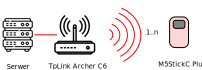
\includegraphics[width=0.8\textwidth]{schemat_polaczenia_w_sieci.png}        
        \caption{Uproszczony schemat sieci}        
        \label{rys:upr-schemat-sieci}
    \end{center}
\end{figure}

\section{Standard sieci bezprzewodowej}
Sieć bezprzewodowa jest oparta na technologii IEEE 802.11, szerzej znanej jako Wi-Fi.
Technologia ta została wybrana jako najtańsza dostępna, wszechstronna i wystarczająca
do wymagań \cite{networking}. 

\begin{figure}
    \begin{center}
        \includegraphics[width=0.4\textwidth]{logo_wifi.png}        
        \caption{Logo technolgoii Wi-Fi}        
    \end{center}
\end{figure}


\section{Adresy i DHCP}
Serwer DHCP umożliwia pominięcie ręcznego ustawiania IP dla węzłów. Jest on niezbędny 
dla poprawnego działania projektu. Urządzenie na którym działa aplikacja serwerowa oraz
serwer NTP mają przydzielone stałe IP, mieszczące się w tej samej sieci co węzły, jednak 
nie mieszczące się w puli DHCP.
\par Dla potrzeb projektu założono, że cały system będzie się mieścił w jednej sieci.
Adres tej sieci to \textbf{192.168.0.0}, natomiast maska to \textbf{255.255.255.0}.
Biorąc pod uwagę, że ostatni adres w sieci jest adresem broadcast, a adres "zerowy"
jest adresem sieci, liczba dostępnych adresów wynosi $2^8-2=254$. Dodatkowo, należy
zarezerwować adresy IP dla routera oraz dla serwrea aplikacji. Przyjmijmy, 
że będą to odpowiednio \textbf{192.168.0.1} oraz \textbf{192.168.0.254}. 
Pozostawia to \textbf{252 adresy} do wykorzytania na rzecz węzłów. 
Zakres adresów DHCP zaczyna się więc na \textbf{192.168.0.2} oraz
kończy na \textbf{192.158.0.253}. Listę adresów w sieci zaprezentowano 
w tabeli \ref{tab:addresses}. Odpowiednią konfigurację routera 
zaprezentowano na rys. \ref{rys:ustawienia-routera}. Konfigurację 
portu sieciowego serwera przedstawiono na rys. \ref{rys:konfig-ip-serwera}.

\begin{table}[ht]
    \centering
    \begin{tabular}{|l | l | l|}
    Adres & Przeznaczenie & Nadany przez DHCP \\
    \hline
    192.168.0.0 & Adres sieci & n/d \\
    192.168.0.1 & Adres routera, brama domyślna & NIE \\
    192.168.0.2...253 & Pula adresów dla węzłów & TAK \\
    192.168.0.254 & Adres serwera & NIE \\
    192.168.0.255 & Adres rozgłoszeniowy & n/d
    \end{tabular}
    \caption{Lista adresów składających się na sieć pomiarową}
    \label{tab:addresses}
\end{table}

\begin{figure}
    \begin{center}
        \includegraphics[width=\textwidth]{ustawienia_dhcp.png}        
        \caption{Ustawienia DHCP w routerze TpLink Archer C6}     
        \label{rys:ustawienia-routera}   
    \end{center}
\end{figure}

\begin{figure}
    \begin{center}
        \includegraphics[width=\textwidth]{server_ustawienia_sieciowe.png}        
        \caption{Ustawienia sieciowe na serwerze}       
        \label{rys:konfig-ip-serwera} 
    \end{center}
\end{figure}

\chapter{Przepływ informacji w sieci}
Inicjowanie połączenia pomiędzy serwerem a węzłami to zadanie węzłów.
Po podłączeniu do sieci, próbują się one połączyć do serwera, do portu 7122.
Port ten został wybrany na podstawie udostępnionej przez organizację IANA
listy portów, gdzie widnieje jako niezarezerwowany.
\cite{iana-ports}

\section{Przyjęte kody żądań i odpowiedzi}
W strukturach wiadomości na różnych etapach komunikacji pojawiają się
kody żądań i odpowiedzi, zdefiniowane unikatowo dla całego systemu. 
Kody zapisane są w jednym bajcie. Przedstawiono je w tabelach 
\ref{tab:request-codes} i \ref{tab:response-codes}

\begin{table}[ht]
    \centering
    \begin{tabularx}{\textwidth}{|l | X | X|}
    Kod & Znaczenie & Etap komunikacji \\
    \hline
    0x01 & Żądanie rejestracji węzła przez wygenerowanie dla niego ID & Nawiązywanie połączenia \\
    0x02 & Żądanie autoryzacji przy użyciu wcześniej nadanego ID & Nawiązywanie połączenia \\
    0x03 & Informacja o przesyłaniu paczki danych przez węzeł do serwera & Wymiana informacji \\
    0x04 & Żądanie zmiany konfiguracji węzła & Polecenia kontrolne \\
    0x05 & Żądanie wstrzymania lub rozpoczęcia pomiarów & Polecenia kontrolne \\
    \end{tabularx}
    \caption{Lista kodów żądań}
    \label{tab:request-codes}
\end{table}

\begin{table}[ht]
    \centering
    \begin{tabularx}{\textwidth}{|l | X | X|}
    Kod & Znaczenie & Etap komunikacji \\
    \hline
    0x01 & Ok: wiadomość odebrana i przetworzona pomyślnie & Każdy \\
    0x02 & Podane ID nie istnieje & Nawiązywanie połączenia \\
    0x03 & Węzeł o podanym ID jest już połączony & Nawiązywanie połączenia \\
    0x04 & Brak wolnych ID w puli & Nawiązywanie połączenia \\
    0x05 & Handshake niepoprawny & Nawiązywanie połączenia \\
    0x06 & Kod żądania nie został rozpoznany & Każdy \\
    0x07 & Niepoprawna struktura nagłówka pakietu danych & Wymiana informacji \\
    0x08 & Niepoprawna struktura treści pakietu danych & Wymiana informacji \\
    0x09 & Pomiar już rozpoczęty & Polecenia kontrolne \\
    0x0A & Pomiar już zatrzymany & Polecenia kontrolne \\
    0x0B & Struktura komendy niepoprawna & Polecenia kontrolne \\
    \end{tabularx}
    \caption{Lista kodów odpowiedzi i błędów}
    \label{tab:response-codes}
\end{table}

\section{Nawiązywanie połączenia}
Nawiązywanie połączenia może przebiegać według kilku scenariuszy. Wśród nich
znajdują się pozytywne, zakończone nawiązaniem połączenia oraz w zależności
od wybranej przez węzeł metody nawiązania połączenia różne negatywne,
zakończone zamknięciem przez serwer połączenia TCP. Ogólny schemat połączenia
pomyślnego zaprezentowano na rys. \ref{rys:conn-happy-path}, natomiast 
ogólny schemat połączenia nieudanego zaprezentowano na rys \ref{rys:conn-sad-path}.
Komunikacja zawsze jest rozpoczynana przez węzeł. Tworzy on połączenie
TCP, a następnie wysyła pakiet handshake. 

\begin{figure}
    \begin{center}
        \includegraphics[width=0.7\textwidth]{handshake_happy_path.png}        
        \caption{Pomyślne nawiązanie połączenia}        
        \label{rys:conn-happy-path}
    \end{center}
\end{figure}

\begin{figure}
    \begin{center}
        \includegraphics[width=0.7\textwidth]{handshake_sad_path.png}        
        \caption{Niepowodzenie w nawiązywaniu połączenia}        
        \label{rys:conn-sad-path}
    \end{center}
\end{figure}

\subsection{Handshake}
Handshake to nazwa dla conajmniej dwóch komunikatów przesyłanych jako
pierwsze po zainicjowaniu połączenia TCP pomiędzy węzłem i serwerem.
Węzeł może poprosić serwer o rejestrację, kiedy nie ma zapisanego
w pamięci, wcześniej nadanego ID. Może też zażądać autoryzacji przy 
użyciu zapisanego ID. Handshake trwa, dopóki węzeł nie zerwie 
połączenia lub serwer pomyślnie nie zautoryzuje węzła, jak zaprezentowano
na rysunkach \ref{rys:conn-happy-path} i \ref{rys:conn-sad-path}.
Strukturę wiadomości w handshake opisano w tabelach \ref{tab:handshake-sensor}
oraz \ref{tab:handshake-server}.

\begin{table}[ht]
    \centering
    \begin{tabularx}{\textwidth}{|X | X | X|}
        \hline
        1 bajt & 1 bajt\\
        \hline
        kod żądania & ID \\
        \hline
        Kod żądania (patrz tab. \ref{tab:request-codes}, etap nawiązywanie połączenia) & ID, jeżeli kod to 0x02, w innym wypadku bez znaczenia \\
        \hline
        \end{tabularx}
        \caption{Struktura wiadomości handshake wysyłanej przez węzeł}
        \label{tab:handshake-sensor}
\end{table}

\begin{table}[ht]
    \centering
    \begin{tabularx}{\textwidth}{|X | X | X|}
    \hline
    1 bajt & 1 bajt\\
    \hline
    kod odpowiedzi & ID \\
    \hline
    Kod odpowiedzi (patrz tab. \ref{tab:response-codes}, etap nawiązywanie połączenia) & ID, jeżeli kod to 0x02 \\
    \hline
    \end{tabularx}
    \caption{Struktura odpowiedzi handshake wysyłanej przez serwer}
    \label{tab:handshake-server}
\end{table}

\section{Komunikacja po nawiązaniu połączenia}
Po pomyślnym nawiązaniu połączenia następuje obustronne wysyłanie wiadomości
pomiędzy węzłem a serwerem. Węzeł ma możliwość, według zasad
obecnie aktywnej konfiguracji, żeby wysyłać do serwera pakiety danych.
Serwer natomiast ma możliwość wysyłać do czujnika polecenia konfiguracji
i przełączania.
\subsection{Wysyłanie pakietów danych}
Wysyłanie pakietów danych przez węzeł odbywa się w regularnych, lub nieregularnych odstępach
czasu, w zależności od czujnika i jego konfiguaracji.
Dane z czujników są zbierane w paczki, które opatrzone odpowiednimi
informacjami w nagłówku są przesyłane do serwera. Serwer nie zwraca potwierdzenia
pomyślnego odebrania danych, choć takie rozwiązanie może być
pomocne w testowaniu
wdrożenia rozwiązań opartych na tym systemie i może stanowić niezbędne
usprawnienie komunikacji w dalszym rozwoju projektu.
\par Długość paczek danych jest zmienna i dla każdego czujnika może być określana indywidualnie.
Przyjęty przez nas maksymalny rozmiar pakietu TCP dla czujnika IMU
wynosi 1460 bajtów. Limit ten jest jednak
umowny i może zostać zmieniony kosztem zwiększenia zajętości pamięci dynamicznej mikroprocesora, 
przez co zminejszy się możliwość rozbudowy systemu. 
Dla mikrofonu rozmiar paczki to 16 bajtów nagłówka plus ilość danych,
która akurat znajdowała się w buforze 
w momencie wysłania pakietu.
\par Struktura pakietu danych składa się z nagłówka oraz treści. 
Treść to zbiór kolejnych odczytów, które są definiowane
przez nagłówek paczki oraz obecne ustawienia czujnika.
Struktura nagłówka została przedstawiona w tabeli \ref{tab:data-pack-header}.
Nagłówek zawiera informacje niezbędne do prawidłowej interpretacji treści.
Na podstawie danych z nagłówka określa się czas wykonania
poszczególnych pomiarów. Pierwszy pomiar został wykonany w 
podanej sekundzie i mikrosekundzie, a kolejne były wykonywane
z podaną w tym nagłówku częstotliwością.

\begin{table}[H]
    \centering
    \begin{tabularx}{\textwidth}{| X | X | X | X | X | X |}
    \hline
    \multicolumn{6}{|c|}{16 bajtów}\\
    \hline
    1 bajt 
    & 1 bajt
    & 4 bajty 
    & 4 bajty
    & 4 bajty 
    & 2 bajty \\
    \hline
    Kod komunikatu (0x03) 
    & Typ danych 
    & Sekundy
    & Mikrosekundy 
    & Częstotliwość 
    & Ilość \\
    \hline
    Kod komunikatu (patrz tab. \ref{tab:request-codes}) 
    & Typ przesyłanych danych: mikrofon lub IMU \ref{tab:command-sensor}
    & Sekundy wykonania pierwszego pomiaru 
    & Mikrosekundy wykonania pierwszego pomiaru 
    & Częstotliwość wykonywania pomiarów 
    & Ilość wykonanych pomiarów (little endian) \\
    \hline
    \end{tabularx}
    \caption{Struktura nagłówka paczki danych}
    \label{tab:data-pack-header}
\end{table}

\begin{table}[H]
    \centering
    \begin{tabularx}{\textwidth}{| X | X |}
    \hline
    \multicolumn{2}{|c|}{1 bajt}\\
    \hline
    kod czujnika
    & czujnik\\
    \hline
    0x01
    & IMU\\
    \hline
    0x02
    & Mikrofon\\
    \hline
    \end{tabularx}
    \caption{Kody czujników w komunikacji}
    \label{tab:command-sensor}
\end{table}

\subsection{Wysyłanie poleceń do węzła}
Pakiety poleceń, a więc żądania wyłączenia, włączenia lub przełączania
czujnika oraz konfiguracji czujników składają się z kilku (conajmniej trzech)
bajtów i są wysyłane przez serwer do węzła. 

\begin{table}[H]
    \centering
    \begin{tabularx}{\textwidth}{| X | X | X |}
    \hline
    \multicolumn{3}{|c|}{3+ bajtów}\\
    \hline
    1 bajt 
    & 1 bajt
    & 1 bajt (lub więcej) \\
    \hline
    Kod polecenia (0x03) 
    & Rodzaj polecenia 
    & Dodatkowe argumenty \\
    \hline
    Kod polecenia (patrz tab. \ref{tab:request-codes}) 
    & Rodzaj polecenia: ustawienia lub przełączenie 
    & Dodatkowe argumenty, jeżeli rodzaj polecenia ich wymaga. Są ne indywidualne dla każdego czujnika. \\
    \hline
    \end{tabularx}
    \caption{Struktura pakietu polecenia}
    \label{tab:command-structure}
\end{table}

\section{Bezpieczeństwo}
\subsection{Bezpieczeństwo danych}
Połączenie pomiędzy węzłem i serwerem pozostaje niezaszyfrowane. 
Bezpieczeństwo danych nie jest wymogiem koniecznym w założeniach
projektu, natomiast jest możliwe jego wprowadzenie, jeżeli bezpieczeństwo
przesyłanych danych stanowi priorytet. Polecanym rozwiązaniem jest 
warstwa TLS, pozwalająca zapewnić autentyczność i bezpieczeństwo 
przesyłanych danych \cite{networking} \cite{khan-tls}. Wprowadzenie
takich modyfikacji będzie wymagało ingerencji w kod oprogramowania serwerowego
oraz oprogramowania węzła, wychodzącej daleko poza zakres tej pracy.


\subsection{Odporność na chwilowe zerwanie połączenia}
Chwilowe zaniki połączenia są obsługiwane przez kartę sieciową serwera
oraz węzłów. Fakt korzystania z protokołu TCP/IP sprawia, że nie
ma potrzeby przykładać wagi do tego problemu z poziomu oprogramowania
aplikacji. 
\par Jeżeli połączenie zostanie
chwilowo zerwane pomiędzy serwerem a węzłem, to próbują one 
nawiązać komunikację raz jeszcze. Węzeł zatrzymuje w tym momencie pracę
i próbuje nawiązać polączenie z serwerem. Jeżeli połączenie
zostanie poprawnie nawiązane i handshake zakończy się sukcesem, to
węzeł wznawia pracę w miejscu w którym nastąpiło przerwanie.


\chapter{Aplikacja serwerowa}
\section{Architektura aplikacji}
Oprogramowanie napisane w języku Go można podzielić na dwa serwisy:
jeden obsługujący połączenie z węzłami, odbierający z nich dane i
zapisujący je, a także wysyłający do nich polecenia oraz drugi, 
odpowiedzialny za interakcję z użytkownikiem lub innym programem 
poprzez interfejs webowy oraz REST API, czyli interfejsu
programisytcznego dla oprogramowania interfejsu użytkownika.
Wewnętrzna szyna danych pozwala na
przekazywanie danych wejściowych (poleceń) od użytkownika do odpowiedniego
węzła. Całościowy obraz systemu został zaprezentowany na rys. \ref{rys:server-app-schema}.
\par Punkt wejściowy programu, który 
jest głównym wątkiem, ma za zadanie
połączyć się z bazą i utworzyć wszystkie 
struktury, które będą wykorzystywane
przez wiele części aplikacji, jak np. obiekt połączenia z bazą, obiekt
rejestr węzłów, szyna danych. 
Następnie tworzy on wątki programu, 
którym przekazuje utworzone wcześniej struktury.
Kod opisujący to zachowanie został załączony
jako \ref*{main.go}.

\begin{figure}[H]
    \begin{center}
        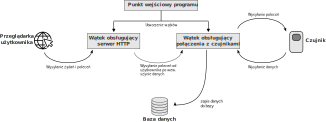
\includegraphics[width=\textwidth]{schemat_architektury_aplikacji_serwerowej.png}        
        \caption{Schemat architektury aplikacji serwerowej}        
        \label{rys:server-app-schema}
    \end{center}
\end{figure}


\subsection{Interakcja z węzłami}
Wątek odpowiedzialny za interakcję z węzłami rozpoczyna się utworzeniem
wątków interpreterów wiadomości. Zostaną one 
wykorzystane później, do zrównoleglenia obsługi danych przychodzących 
z różnych węzłów. Potem następuje otwarcie
nasłuchu na porcie 7122. Jeżeli połączenie TCP/IP zostanie nawiązane, to
utworzony zostaje kolejny wątek obsługujący to połączenie, a sam wątek 
macierzysty wraca do nasłuchiwania. Nowy wątek oczekuje od węzła
wiadomości handshake. Kod odpowiedzialny
za interpretację wiadomości handhsake jest
załączony jako \ref*{handshake.go}. Po pomyślnym handshake tworzony jest osobny wątek 
przesyłający polecenia do węzła, jeżeli jakieś się pojawią, a sam
wątek macierzysty rozpoczyna obsługę danych
przychodzących z węzła w pętli. 
Zachowanie zostało przedstawione na rys. \ref{rys:server-sensor-flow},
kod wątku został załączony jako \ref*{listen.go}, 
a kod odpowiedzialny za odbiór wiadomości
jako \ref*{receiver.go}.
\par W przypadku zakończenia pracy wątku obsługującego połączenie usuwane
są wszystkie wątki przez niego utworzone, natomiast główny wątek 
tworzący wątki interpreterów jest kończony tylko kiedy
główny program zostanie zakończony. 

\begin{figure}[H]
    \begin{center}
        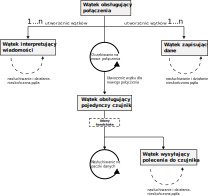
\includegraphics[width=0.8\textwidth]{schemat_watkow_obslugi_czujnikow.png}        
        \caption{Schemat wątków obsługi węzłów}        
        \label{rys:server-sensor-flow}
    \end{center}
\end{figure}

\subsection{Interakcja z użytkownikiem}
Użytkownik może wchodzić w inteakcje z aplikacją, to znaczy wysyłać polecenia
rekonfiguracji do wybranych węzłów. Możliwe jest to dzięki modułowi aplikacji
odpowiedzialnemu za serwer HTTP. Serwer udostępnia interfejs użytkownika
oraz REST API, z którego interfejs użytkownika korzysta. 
\par Zadaniem serwera HTTP jest odbieranie i wysyłanie żądań 
protokołu HTTP i HTTPS, czyli szyfrowanych. W naszym 
przypadku połączenie będzie 
niezaszyfrowane, choć możliwe jest jego zaszyfrowanie przy pomocy
dedykowanego oprogramowania, np. serwera Nginx. 
\cite{wikipedia:web-server} \cite{nginx-tls}
\par Interfejs użytkownika, zawarty w katalogu projektu poświęconym aplikacji
serwerowej \texttt{server/gui}
jest utworzony na podstawie HTML, CSS oraz
JavaScript. Jest on opisany na wielu plikach, rozdzielonych 
według swojego przeznaczenia (struktura, stylowanie, skrypt). 
W przypadku HTML i CSS do stylizacji został wykorzystany
framework Bootstrap, czyli zestaw gotowych komponentów, pozwalający
skrócić pracę i uzyskać pewność estetyki \cite{bootstrap}.
 W przypadku JavaScript, czyli
języka odpowiedzialnego za skrypty i mechanikę interfejsu, użyto
frameworka Vue. \cite{vue} Sam serwer HTTP został zbudowany na
bazie frameworka Gin. \cite{gin} Architektura rozwiązania po stronie
serwera, w więc z pominięciem interfejsu użytkownika, została
przedstawiona na rys. \ref{rys:server-http-flow}.
Kod kontrolera, odpowiedzialny za odebranie
od użytkownika danych nt komend, które
mają zostać przekazane do czujnika załączono
jako \ref*{command.go}.

\begin{figure}[H]
    \begin{center}
        \includegraphics[width=0.15\textwidth]{logo_html.png}        
        \caption{Logo technolgoii HTML}        
        \label{rys:logo-html}
    \end{center}
\end{figure}

\begin{figure}[H]
    \begin{center}
        \includegraphics[width=0.15\textwidth]{logo_gin.png}        
        \caption{Logo frameworka Gin}        
        \label{rys:logo-gin}
    \end{center}
\end{figure}

\begin{figure}[H]
    \begin{center}
        \includegraphics[width=0.15\textwidth]{logo_css.png}        
        \caption{Logo technologii CSS}        
        \label{rys:logo-css}
    \end{center}
\end{figure}

\begin{figure}[H]
    \begin{center}
        \includegraphics[width=0.15\textwidth]{logo_vue.png}        
        \caption{Logo frameworka Vue}        
        \label{rys:logo-vue}
    \end{center}
\end{figure}

\begin{figure}[H]
    \begin{center}
        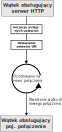
\includegraphics[width=0.3\textwidth]{schemat_serwisu_http.png}        
        \caption{Schemat części aplikacji obsługującej serwer HTTP}        
        \label{rys:server-http-flow}
    \end{center}
\end{figure}

\subsection{Przepływ informacji i zapis danych}

W procesie tworzenia aplikacji wypróbowano wiele metod 
zapisu danych z czujników, spośród których najwydajniejszy okazał
się zapis binarny do plików. Baza danych, do której następują odwołania w 
pracy to po prostu 
system plików serwera. Odczyty z czujników są zapisywane do plików binarnych.
Taki porządek rzeczy jest podyktowany stosunkowo niskim kosztem zapisu
danych w tym formacie w porównaniu do innych, wypróbowanych rozwiązań,
jednak taki zapis wprowadza konieczność późniejszego (po zakończonym pomiarze 
i zapisie) przetworzenia plików na format zdatny do analizy. Proces ten
został opisany w podrozdziale \ref*{file-parsing-chapter}.
Na wcześniejszym etapie rozwoju projektu została zastosowana baza 
relacyjna MySQL, a po niej zapis bezpośrednio do plików CSV, 
jednak te metody okazały się zbyt nieprzystosowane
do zapisywania tak dużej liczby danych w tak małym czasie, w 
efekcie czego następowało gubienie pomiarów oraz wyoskie zużycie zasobów
serwera. 
\begin{figure}[H]
    \begin{center}
        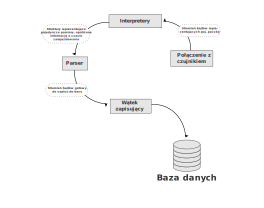
\includegraphics[width=\textwidth]{schemat_przeplywu_zapisu_danych.png}        
        \caption{Schemat przepływu informacji zapisywanych do bazy danych}        
        \label{rys:database-save-flow}
    \end{center}
\end{figure}
\par Schemat przepływu informacji
został zaprezentowany na rys. \ref{rys:database-save-flow}.
Żaden wątek obsługujący połączenie z węzłem nie dokonuje zapisu
do bazy bezpośrednio. Ciąg bajtów reprezentujący jeden pakiet pomiarów
jest przekazywany przez wątek obsługujący połączenie z węzłem do kolejki
interpreterów, która jest obsługiwana przez pulę wątków 
interpretujących wiadomości. To zachowanie jest widoczne w 
kodzie obsługującym nasłuch, załączonym
jako \ref*{listen.go}, a kod wątków interpretujących
został załączony jako \ref*{interpreter.go}. 
Ich zadaniem jest na podstawie otrzymanych w nagłówku pakietu informacji
podzielenie ciągu na pojedyncze pomiary oraz określenie czasu
ich zarejstrowania. Tak przygotowane struktury są wysyłane do kolejki 
parserów, gdzie są zamieniane na ciągi bajtów w takiej formie, 
w jakiej mają trafić do pliku. Następnie te dane są kierowane do
kolejki zapisów, gdzie wątek zapisujący dane zajmuje się zapisem danych
do bazy.
Kod odpowiedzialny za zapis danych oraz parsowanie struktur załączono
jako \ref*{readings.go}.
\par Informacja o węzłach w aplikacji sprowadza się tylko do 
listy ID węzłów, które zostały wydane oraz listy ID, które są 
obecnie połączone. Dane te są ulotne, trzymane w pamięci programu. 
Dobrym kierunkiem dalszego rozwoju jest umieszczenie ich w bazie 
danych, a także zbieranie dodatkowych informacji jak np. unikalny
identyfikator (MAC) urządzenia do którego ID należy, obecnie
aktywne ustawienia etc.

\subsection{Przekazywanie poleceń od użytkownika do węzła}
Wewnętrzna szyna danych jest oparta na wzorcu projektowym obserwator,
którego ogólny schemat w notacji UML został przedstawiony 
na rys \ref{rys:schemat-obserwator} \cite{gof-patterns}.
Oprócz tego, opiera się ona również na wbudowanych w język
strukturach danych, kanałach (ang. channel), będących implementacją
kolejek, bezpiecznych do używania w środowisku wielowątkowym 
\cite{blue-book}.
Jej zadaniem jest przekazywanie poleceń od użytkownika, wprowadzonych
za pomocą interfejsu webowego do konkretnych węzłów, których 
te polecenia dotyczą.
\par W głównym wątku programu jest inicjalizowana struktura
- szyna danych, 
zawierająca odniesienie to wektora kanałów. Isnieje metoda, 
pozwalająca na dodanie do wektora nowego kanału oraz zwracająca
wskaźnik do niego. Za każdym razem, kiedy zostanie wysłana
wiadomość z poleceniem na szynę danych, jest ona przekazywana
dalej do każdego z kanałów w tym wektorze, jest to 
tzw. broadcast. Odbiorcy tych kanałów, w domyśle wątki 
obsługujące komunikację z węzłem już we własnym  zakresie
decydują, czy otrzymana wiadomość powinna zostać wysłana do
węzła na podstawie załączonego do wiadomości ID. Działanie
tego systemu zostało zobrazowane na rys. \ref{rys:schemat-szyny-danych}.
Kod szyny został załączony do pracy jako \ref*{exchange.go}

\begin{figure}[H]
    \begin{center}
        \includegraphics[width=0.5\textwidth]{schemat_obserwator.png}        
        \caption{Ogólny schemat wzorca obserwator w graficznej reprezentacji notacji UML}        
        \label{rys:schemat-obserwator}
    \end{center}
\end{figure}

\begin{figure}[H]
    \begin{center}
        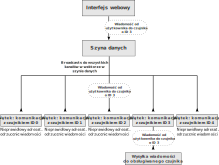
\includegraphics[width=0.8\textwidth]{schemat_szyny_danych.png}        
        \caption{Schemat działania szyny danych}        
        \label{rys:schemat-szyny-danych}
    \end{center}
\end{figure}


\section{Wydajność i ograniczenia}
Liczba wątków interpretujących jest konfigurowalna,
może zostać dostosowana do bieżących potrzeb. Aplikacja po drobnych
modyfikacjach
nadaje się do skalowania horyzontalnego, czyli zwiększania wydajności
programu poprzez uruchamianie jej na dodatkowych maszynach. Wymagany
byłby do tego load balancer \cite{load-balancer}. Testy wydajności oraz badanie 
ograniczeń aplikacji przeprowadzono dla jednej maszyny, z węzłami
połączonymi w sieci lokalnej. Specyfikacja maszyny, zawierająca
najważniejsze informacje, została przedstawiona w tabeli 
\ref{tab:specyfikacja-maszyny} \cite{dell-specs}. Pozostałe elementy użyte w
testach są tymi samymi, które wymieniono w rozdziale poświęconym
użytym elementom.
\par Testy rozpatrują ograniczenia na poszczególnych etapach
komunikacji. Dla danej konfiguracji, maksymalna wydajność całego
systemu ograniczona jest przez ten element, którego możliwości przetwarzania
lub przesyłania danych będą najniższe, tzw. "wąskie gardło".
\begin{table}[ht]
    \centering
    \begin{tabularx}{\textwidth}{|X | X | X|}
        \hline
        Element systemu & Specyfikacja\\
        \hline
        Procesor &  Intel(R) Core(TM) i5-7300HQ CPU @ 2.50GHz, 4 rdzenie \\ 
        \hline
        Karta sieciowa & Realtek Semiconductor Co., Ltd. RTL8111/8168/8411 PCI Express \\ 
        \hline
        Pamięć RAM & 16 GB DDR4 \\ 
        \hline
        Dysk twardy & Samsung SSD 970 EVO 250GB \\ 
        \hline
        \end{tabularx}
        \caption{Specyfikacja maszyny, użytej do testów wydajności i ograniczeń}
        \label{tab:specyfikacja-maszyny}
\end{table}

\subsection{Wydajność węzła i specyfikacja danych wejściowych}
Karta sieciowa węzła nie pozwala na wysłanie większej ilości
danych niż 1 MB/s. Węzeł nie jest w stanie wygenerować tyle 
danych, aby ten bufor zapełnić. Doświadczalnie wyznaczono, że
przy największej instensytnowści pracy (mikrofon, 44100 Hz)
pojedynczy węzeł przesyła dane z prędkością nie większą niż
100 kB/s.

\subsection{Wydajność routera}
W zależności od użytego routera, jego wydajność będzie się
zmieniać. Użyty do testów router to TpLink Archer C6,
którego złącza przewodowe pracują z prędkością do 125 MB/s
oraz który ma możliwość pracy w standardzie 
Wi-Fi 802.11ac. Maksymalna teoretyczna przepustowość dla
częstotliwości 2,4 GHz, w której pracują karty sieciowe
węzłów wynosi 37,5 MB/s. Przepustowość sieci 
bezprzewodowej jest dzielona pomiędzy podłączone urządzenia. 
Jeżeli przyjmiemy, że jeden czujnik potrzebuje 
przepustowości 100 kB/s, to z użyciem tego urządzenia możliwe
jest efektywne wykorzystanie do 375 czujników.

\subsection{Wydajność karty sieciowej serwera}
Karta sieciowa na serwerze obsługuje do 125 MB/s na połączeniu
kablowym. Ta wartość jest podobna do obsługiwanej przez 
router, co sprawia, że karta sieciowa używana w testowanej sieci
nie będzie ogarniczeniem - nie będzie zmuszona do przetwarzania 
większej ilości danych, niż te dostarczone przez router.

\subsection{Wydajność aplikacji serwerowej}  \label{app-efficiency-subsection}
Aplikacja serwerowa została przetestowana pod względem wykorzystywanych
zasobów serwera z każdą dostępną ilością czujników, z każdym rodzajem
czujnika. Pomiaru dokonano za pomocą narzędzia 'docker stats', na
uruchomionej, skonteneryzowanej aplikacji z udostępnionym odpowiednim
portem. Zużycie CPU jest mierzone w procentach czasu obliczeniowego
oferowanego przez jeden rdzeń procesora, co oznacza, że wyniki 
powyżej 100\% są możliwe, gdyż oznacza to wykorzystanie 
czasu obliczeniowego więcej niż jednego rdzenia. W stanie bezczynności, tj.
żadne pomiary nie są wykonywane, aplikacja serwerowa zajmuje
0\% CPU oraz 6,5 MB RAMu.
Pomiary zużycia zasobów zostały zaprezentowane w tab. \ref*{tab:zestawienie-wydajnosci}.
Zauważyć można, że wzrost zużycia pamięci oraz czasu obliczeniowego
procesora jest liniowy, co jest spodziewanym zjawiskiem - każdy czujnik 
dodaje dwa wątki obsługujące połączenie (wysyłanie komend, odbieranie danych)
oraz dodaje stałą liczbę pakietów odbieranych przez serwer.

\begin{table}[H]
    \centering
    \begin{tabularx}{\textwidth}{|X | X | X|}
        \hline
        Konfiguracja & użycie CPU [\%$\pm$0,1\%] & Użycie RAM [MB$\pm$0,1MB]\\
        \hline
        Jeden czujnik IMU & 1,2 & 15,4 \\
        \hline
        Dwa czujniki IMU & 1,6 & 19,1 \\ 
        \hline
        Trzy czujniki IMU & 3,1 & 25 \\ 
        \hline
        Cztery czujniki IMU & 4,3 & 31,2 \\ 
        \hline
        Jeden czujnik MIC & 13 & 25 \\ 
        \hline
        Dwa czujniki MIC & 20,1 & 28,9 \\ 
        \hline
        Trzy czujniki MIC & 35 & 36,1 \\ 
        \hline
        Cztery czujniki MIC & 44,8 & 49,3 \\ 
        \hline
        \end{tabularx}
        \caption{Zestawienie zużycia zasobów przez aplikację działającą w pełnej wersji}
        \label{tab:zestawienie-wydajnosci}
\end{table}

\section{Interfejs webowy}
Spośród różnych możliwości, jak np. interakcja przez konsolę czy
natywna aplikacja okienkowa na komputery, wybrany został interfejs
webowy, dostępny przez przeglądarkę. Wybór taki jest najlepszy z
podanych, ponieważ zapewnia łatwość i prostotę implementacji i 
użytkowania. Nie wymaga instalowania dedykowanego oprogramowania 
a jedynie posiadania przeglądarki z dostępem do odpowiedniego
portu serwera aplikacji. W niczym również nie ustępuje alternatywnym
rozwiązaniom.

\subsection{REST API}
REST API zapewnia interfejsowi webowemu oraz programistom dalej
rozbudowującym komunikację z aplikacją zestaw narzędzi, przeznaczonych
do komunikacji z  aplikacją \cite{rest-api}. API opiera się na formacie danych JSON, 
który stanowi najlepszy wybór do tego typu komunikacji ze względu
na swoją prostotę i klarowność. Obecnie REST API jest ograniczone
do endpointu POST $/command$ (np. http://localhost:8081/command),
 czyli adresu, na który należy wysłać 
żądanie HTTP, który przyjmuje dane w metodzie POST i 
pozwala na wysyłanie poleceń do węzłów. Użytkownik nie musi robić tego ręcznie, 
jest to automatycznie robione przez skrypty interfejsu użytkownika. 
W przyszłości można 
rozbudować API o endpointy pozwalające na pobranie danych nt węzłów
czy stanu serwera.

\subsection{Interfejs HTML i JavaScript}
Interfejs webowy, napisany przy użyciu HTML, CSS i JavaScript oraz
odpowiednich dla tych języków frameworków stanowi przykład standardowego
panelu kontrolnego, dostępnego przez internet. Interfejs
zaprezentowany został na rys. \ref{rys:web-interface}.
Jest to prosty zestaw pól typu select oraz różnych przycisków, 
pozwalających na wysłanie ustawionych danych do serwera
a także lista komunikatów walidacyjnych. Przyciski oskryptowane
są w taki sposób, że na naciśnięcie wysyłają do serwera polecenie,
w którym są wyspejalizowane, zbierając przy tym wartości 
wskazane w panelu. Działanie skryptu zostało zaprezentowane 
na rys. \ref{rys:frontend-script-schema}

\begin{figure}[H]
    \begin{center}
        \includegraphics[width=\textwidth]{interfejs_webowy.png}
        \caption{Interfejs webowy, panel kontrolny systemu}        
        \label{rys:web-interface}
    \end{center}
\end{figure}

\begin{figure}[H]
    \begin{center}
        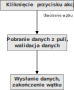
\includegraphics[width=0.4\textwidth]{schemat_interfejsu_webowego.png}
        \caption{Schemat przedstawiający działanie skryptu w interfejsie webowym}        
        \label{rys:frontend-script-schema}
    \end{center}
\end{figure}

\chapter{Aplikacja węzłów}
\section{Architektura aplikacji}
Architektura aplikacji węzłów została zaprezentowana na rys.\ref{rys:architektura-aplikacji-węzłów}.
Aplikację można podzielić na 2 główne części. Część główna aplikacji, odpowiada za:

\begin{itemize}
    \item logowanie się do sieci Wi-Fi
    \item nawiązywanie/odawianie połączenia z aplikacją serwerową i wysyłanie danych
    \item odbieranie komend od aplikacji serwerowej i ich wykonanie ich
\end{itemize}

Część pomiarowa aplikacji, składa się z modułów, po jednym dla każdego czujnika.
Każdy moduł jest samodzielną częścią aplikacji, która odpowiada za:

\begin{itemize}
    \item odczyt danych z czujnika
    \item przetworzenie danych
    \item wysłanie danych do głównej części aplikacji
\end{itemize}

W celu zapewnienia stabilności czasowej pomiarów, przyjęto że część główna aplikacji
działa na innym rdzeniu niż część pomiarowa. Zapewnia to niezakłócone pomiary, ze stałą częstotliwością.
Niezależnie od stanu głównej aplikacji. Dodatkowym atutem takiego podziału jest możliwość wysyłania danych
do aplikacji serwerowej równole do odczytu kolejnych danych z czujników. 
\par Interakcja pomiędzy obiema częściami aplikacji odbywa się za pomocą kolejek danych \cite{wiki-queue}.
oraz kilku funkcji udostępnionych przez moduły czujników. Za pomocą kolejek danych przesyłane są dane z czujników
do głównej części aplikacji, która następnie przesyła je do aplikacji serwerowej. Każdy moduł czujnika 
do poprawnej integracji z główną częścią aplikacji musi udostępnić funkcje:

\begin{itemize}
    \item inicjalizacji wątku pomiarowego - przyjmuje jako argument wskaźnik na 
    obiekt komunikacyjny, który pozwala dodać wiadomość do kolejki danych
    \item zakończenia wątku pomiarowego - brak argumentów
    \item zmiany parametrów pomiaru - przyjmuje ciąg bajtów, który zawiera parametry pomiaru
\end{itemize}

Natomiast główna część aplikacji udostępnia części pomiarowej funkcję przekazującą dane do kolejki.
Z której następnie zostaną pobrane przez główną część aplikacji i przesłane do aplikacji serwerowej.
\par Przyjęto konwęcję że każdy moduł czujnika przesyła pakiet danych pomiarowych po przez kolejkę w formie
struktury Msg \ref{rys:uc-msg} zdefiniowanej globalnie, która zawiera:

\begin{itemize}
    \item wskaźnik na ciąg bajtów zawierający dane
    \item liczbę wysyłanych bajtów
    \item wskaźnik na mutex który jest zablokowany i zostanie odblokowany po zakończeniu przetwarzania danych
\end{itemize}

\par Taka architektura pozwala na łatwe dodawanie nowych czujników, bez konieczności modyfikacji głównej części aplikacji.\\
\\Kod źródłowy aplikacji znajduje się w \hyperref[node-coode]{Dodatku A}.


\begin{figure}[H]
    \begin{center}
        \includegraphics[width=0.4\textwidth]{uc-msg}
        \caption{Struktura Msg}
        \label{rys:uc-msg}
    \end{center}
\end{figure}

\begin{figure}[H]
    \begin{center}
        \includegraphics[width=0.75\textwidth]{uc-architecture}
        \caption{Architektura aplikacji węzłów}        
        \label{rys:architektura-aplikacji-węzłów}
    \end{center}
\end{figure}

\section{Użyte biblioteki}

\begin{itemize}
\item \textbf{Arduino\cite{arduinoh}} - biblioteka zmienia nasz projekt, dodając nam możliwość
    budowania go analogicznie jak w środowisku Arduino IDE \cite{arduino}. Dzięki temu dostajemy dostęp
    do wielu funkcji, które są dostępne w tym środowisku. 
\item \textbf{WiFi\cite{wifi-h}} - biblioteka umożliwiająca połączenie z siecią Wi-Fi. Dostępna
    jedynie w połączeniu z biblioteką Arduino.
\item \textbf{EEPROM\cite{eeprom.h}} - biblioteka używa pamięci Flash do emulacji pamięci EEPROM. Dostępna
    jedynie w połączeniu z biblioteką Arduino. Używamy jej do zapisywania ID otrzymanego od serwera w
    pamięci nieulotnej.
\item \textbf{M5StickCPlus\cite{m5stick.h}} - biblioteka stworzona przez twórców modułu M5StickC PLUS. Dostępna jedynie
    w połączeniu z biblioteką Arduino. Zawiera biblioteki potrzebne do obsługi
    urządzeń znajdujących się w module. Potrzebujemy
    jedynie części odpowiedzialnej za obsługę modułu zasilającego te urządzenia.
\item \textbf{Wire\cite{wire.h}} - biblioteka odpowiedzialna za łączenie się po przez protokół I2C. 
    Dostępna jedynie w połączeniu z biblioteką Arduino. Używamy jej do komunikacji z 6-cio osiowym IMU.
\item \textbf{driver/i2s\cite{driver.h}} - biblioteka odpowiedzialna za łączenie się po przez protokół I2S. 
    Używamy jej do komunikacji z mikrofonem cyfrowym.
\end{itemize}

\section{Schematy działania aplikacji}

\begin{figure}[H]
    \begin{center}
        \includegraphics[width=0.25\textwidth]{uc-init}
        \caption{Inicjalizacja aplikacji - Dodatek A.1}        
        \label{rys:uc-init}
    \end{center}
\end{figure}

\begin{figure}[H]
    \begin{center}
        \includegraphics[width=0.25\textwidth]{uc-main_task}
        \caption{Główny wątek aplikacji - Dodatek A.1}
        \label{rys:uc-main_task}
    \end{center}
\end{figure}

\begin{figure}[H]
    \begin{center}
        \includegraphics[width=0.2\textwidth]{uc-led_task}
        \caption{Wątek led\_task - \ref*{main.cpp}}
        \label{rys:uc-led_task}
    \end{center}
\end{figure}

\begin{figure}[H]
    \begin{center}
        \includegraphics[width=0.2\textwidth]{uc-send_task}
        \caption{Wątek send\_task - \ref*{main.cpp}}
        \label{rys:uc-send_task}
    \end{center}
\end{figure}

\begin{figure}[H]
    \begin{center}
        \includegraphics[width=0.6\textwidth]{uc-command_function.jpeg}
        \caption{Funkcja przetwarzająca komendy - \ref*{main.cpp}}
        \label{rys:uc-command_function}
    \end{center}
\end{figure}

\begin{figure}[H]
    \begin{center}
        \includegraphics[width=0.2\textwidth]{uc-start_task}
        \caption{Funkcja startująca wątek pomiarowy - \ref*{mpu.cpp} i \ref*{mike.cpp}}
        \label{rys:uc-start_task}
    \end{center}
\end{figure}

\begin{figure}[H]
    \begin{center}
        \includegraphics[width=0.2\textwidth]{uc-end_task.jpeg}
        \caption{Funkcja kończąca wątek pomiarowy - \ref*{mpu.cpp} i \ref*{mike.cpp}}
        \label{rys:uc-end_task}
    \end{center}
\end{figure}

\begin{figure}[H]
    \begin{center}
        \includegraphics[width=0.6\textwidth]{uc-measurement_task}
        \caption{Wątek pomiarowy - \ref*{mpu.cpp} i \ref*{mike.cpp}}
        \label{rys:uc-measurement_task}
    \end{center}
\end{figure}

\begin{figure}[H]
    \begin{center}
        \includegraphics[width=0.4\textwidth]{uc-handshake}
        \caption{Handshake - \ref*{link.cpp}}
        \label{rys:uc-handshake}
    \end{center}
\end{figure}

\begin{figure}[H]
    \begin{center}
        \includegraphics[width=0.2\textwidth]{uc-data-flow}
        \caption{Przepływ danych}
        \label{rys:uc-data-flow}
    \end{center}
\end{figure}

\section{Debugowanie}
\subsection{Separacja kodu debugowego od kodu produkcyjnego}

Aby umożliwić łatwe przełączanie się pomiędzy kodem produkcyjnym a kodem debugowym. Zostało
stworzone makro \ref{rys:uc-makro-cpp} oraz zmienna globalna "DEBUG". Jeżeli zmienna ta ma wartość
0 to kod wewnątrz makra nie jest kompilowany. Jeżeli zmienna ma wartość 1 to kod wewnątrz makra
jest kompilowany. W ten sposób można łatwo przełączać się pomiędzy kodem produkcyjnym a kodem
debugowym. W trybie debugowym można podglądać logi poprzez REPL \ref{rys:uc-repl} po kliknięciu w Visual Studio Code
\ref{rys:vsc-monitor}. Było to pomocne głównie przy sprawzaniu poprawności działania funkcji,
czy logiki aplikacji. Zaimplementowany kod debugowy pozwala:

\begin{itemize}
    \item Sprawdzić IP nadane przez router.
    \item Status połączenia z siecią Wi-Fi.
    \item Status połączenia z serwerem.
    \item Status synchronizacji czasu z serwerem NTP.
    \item Podejrzeć rzebieg komunikacji z serwerem.
    \item Zobaczyć czy handshake przebiegł poprawnie i z jakim ID pracuje węzeł.
    \item Zobaczyć stan aplikacji (Stan jałowy/Stan pomiarowy) oraz który czujnik jest aktywny.
\end{itemize}

Dodatkowo REPL wyświetla informacje o błędach, jeżeli wystąpią.

\begin{figure}[H]
    \begin{center}
        \includegraphics[width=0.25\textwidth]{makro-cpp}
        \caption{Makro debugowe.}
        \label{rys:uc-makro-cpp}
    \end{center}
\end{figure}

\begin{figure}[H]
    \begin{center}
        \includegraphics[width=0.65\textwidth]{makro-cpp-use}
        \caption{Sposób użycia makra debugowego. Tekst zostanie wydrukowany tylko wtedy gdy zmienna DEBUG ma wartość 1.}
        \label{rys:uc-makro-cpp-use}
    \end{center}
\end{figure}

\begin{figure}[H]
    \begin{center}
        \includegraphics[width=0.4\textwidth]{uc-repl}
        \caption{Logi debugowe widoczne poprzez REPL}
        \label{rys:uc-repl}
    \end{center}
\end{figure}

\begin{figure}[H]
    \begin{center}
        \includegraphics[width=0.7\textwidth]{vsc-monitor.png}
        \caption{Przycisk uruchamiający REPL. Widoczny na dolnym pasku narzędzi w Visual Studio Code.}
        \label{rys:vsc-monitor}
    \end{center}
\end{figure}

\subsection{Debugowanie z użyciem Pythona}

W celu debugowania aplikacji został stworzony skrypt w języku Python. Skrypt ten pozwala na
wysyłanie komend do aplikacji. Pozwala on również
na wyświetlenie danych pomiarowych na animowanych wykresach, w czasie rzeczywistym. Ponieważ aplikacja węzłów
powstawała równolegle do aplikacji serwerowej, było to istotne narzędzie, pozwalające sprawdzać poprawność
działania aplikacji węzłów niezależnie od statusu prac nad aplikacją serwerową. Na poniższych rysunkach przedstawiono
screen z działania skryptu.\\
Środowisko na którym pracowano:
\begin{itemize}
    \item Komputer z systemem Linux Ubuntu 22.04
    \item Zainstalowany Python w wersji 3.9.14
    \item Dostęp do sieci internet (do pobrania bibliotek)
\end{itemize}
Aby skonfigurować środowisko debugowe należy otworzyć terminal w folderze "M5StickC/device/test".
A następnie uruchomić poniższe komendy:
\begin{itemize}
    \item sudo apt install python3-tk (środowisko graficzne, wymagane do wyświetlania wykresów)
    \item python3.9 -m venv venv (środowisko wirtualne)
    \item source venv/bin/activate (aktywacja środowiska wirtualnego)
    \item pip install -U pip (aktualizacja pip)
    \item pip install -r requirements.txt (instalacja bibliotek)
\end{itemize}
Aby uruchomić środowisko debugowe należy otworzyć terminal w folderze "data\_test".
A następnie uruchomić poniższą komendy:

\begin{itemize}
    \item source venv/bin/activate
    \item python test\_tool.py
\end{itemize}

\begin{figure}[H]
    \begin{center}
        \includegraphics[width=0.65\textwidth]{pytestmic}
        \caption{Na górze - prezentacja pomiarów z mikrofonu, żyroskopu, oraz akcelerometru. Na dole - logi debugowe.}
        \label{rys:uc-pytest}
    \end{center}
\end{figure}

\subsection{Debugowanie z użyciem Wiresharka}

Podczas integracji systemu z serwerem, zastosowano narzędzie Wireshark do debugowania komunikacji.
Wireshark to wiodąca na świecie aplikacja pozwalająca na podglądanie protokołów sieciowych na niskim poziomie.
Jest to projekt zapoczątkowany przez Geralda Combsa w 1998 roku i do tej pory kontynuowany przez
wielu expertów z całego świata. \cite{wireshark}
\par Wireshark pozwala na podglądanie komunikacji w czasie rzeczywistym. Dzięki temu mogliśmmy zobaczyć czy pakiety są gubione,
czy są wysyłane w odpowiedniej kolejności i formacie. Pozwoliło nam to również znaleźć i usunąć błąd w działaniu systemu.\\
Błędy "TCP window full" oraz "TCP ZeroWindow" \ref{rys:uc-wireshark2} oznaczają że bufor TCP odbiorcy został zapełniony oraz długość okna TCP zostaje ustawiona na zero.
Z reguły dzieje się tak w przypadku, gdy odbiorca nie jest w stanie odebrać danych w odpowiednim tempie \cite{wireshark-zerowindow}. W naszym przypadku
również tak było. Rozwiązaniem problemu było zmienienie architektury programu serwera z synchronicznej na asynchroniczą, oraz zmiana
formatu zapisu danych z MySQL na pliki .csv.

\begin{figure}[H]
    \begin{center}
        \includegraphics[width=0.2\textwidth]{wiresharklogo}
        \caption{Logo aplikacji Wireshark}
        \label{rys:uc-wiresharklogo}
    \end{center}
\end{figure}

\begin{figure}[H]
    \begin{center}
        \includegraphics[width=1\textwidth]{wireshark1}
        \caption{Ramka danych pomiarowych z IMU widoczna w aplikacji Wireshark.
        Aby uzyskać logi nalezy uruchomić aplikację, wybrać sieć w której pracują czujniki i kliknąć 
        interesujący nas pakiet. Dodatkowo możemy przefiltrować pakiety, np po adresie IP, wpisując
        w polu filtra (zielony pasek) "ip.address == adres IP serwera, lub czujnika".}
        \label{rys:uc-wireshark1}
    \end{center}
\end{figure}

\begin{figure}[H]
    \begin{center}
        \includegraphics[width=1\textwidth]{wireshark2}
        \caption{Debugowanie błędów związanych z wydajnością systemu 
        we wczesnych etapach projektu, za pomocą aplikacji Wireshark.}
        \label{rys:uc-wireshark2}
    \end{center}
\end{figure}

\section{Modułość i skalowalność}

Jednym z założeń przyświecających projektowi było zapewnienie modułowości i skalowalności systemu.
Aby to osiągnąć jako część sprzętową wykorzystano moduł pozwalający na wygodne podączanie kolejnych
czujników poprzez wbudowane złacze 2.54mm. Mnogość dostępnych protokołów komunikacyjnych w ESP32
pozwala na łatwe dopasowanie się do potrzeb każdego projektu. Ciekawym rozwiązaniem jest możliwość
podłączenia modułu do sieci CAN \cite{esp32-can}, dzięki czemu można wykorzystać istniejące rozwiązania komunikacyjne
w systemach pojazdów.
\par Od strony programowej, aby dołożyć do projektu nowy czujnik, wystarczy stworzyć moduł programowy
który spełnia wymagania określone w wypracowanym w ramach projektu interfejsie. Dodać numer czujnika do
struktury "Devices" w pliku "globals.hpp" (Dodatek A.3) oraz zarejestrować w głównej części aplikacji w pliku "main.cpp" (Dodatek A.1)
Funkcje startującą wątek pomiarowy \ref{rys:uc-dev-on}, zatrzymującą wątek pomiarowy \ref{rys:uc-dev-off}
oraz ustawiającą parametry modułu \ref{rys:uc-dev-set} według
zamieszczonych w kodzie przykładów.\\
Aplikacja główna wraz z dwoma czujnikami użytymi w projekcie zajmuje 12.2\% pamięci RAM oraz 53.5\% pamięci FLASH \ref{rys:uc-memory}. Co
jest zadowalającym wynikiem, ponieważ pozostawia dużo miejsca na nowe funkcjonalności.

\begin{figure}[H]
    \begin{center}
        \includegraphics[width=0.6\textwidth]{uc-memory}
        \caption{Część logu kompilacji mówiąca o zajętości pamięci.}
        \label{rys:uc-memory}
    \end{center}
\end{figure}

\begin{figure}[H]
    \begin{center}
        \includegraphics[width=0.6\textwidth]{uc-dev-on}
        \caption{Rejestracja funkcji uruchamiających wątki pomiarowe. \ref*{main.cpp}}
        \label{rys:uc-dev-on}
    \end{center}
\end{figure}

\begin{figure}[H]
    \begin{center}
        \includegraphics[width=0.6\textwidth]{uc-dev-off}
        \caption{Rejestracja funkcji kończących wątki pomiarowe. \ref*{main.cpp}}
        \label{rys:uc-dev-off}
    \end{center}
\end{figure}

\begin{figure}[H] 
    \begin{center}
        \includegraphics[width=0.6\textwidth]{uc-dev-set}
        \caption{Rejestracja funkcji ustawiających parametry modułów pomiarowych. \ref*{main.cpp}}
        \label{rys:uc-dev-set}
    \end{center}
\end{figure}

\chapter{Testy systemu pomiarowego}

\section{Proces zbierania danych}
Do testów IMU użyliśmy czterech połączonych ze sobą mechanicznie węzłów.
Pierwszy test polegał na umieszczeniu czujników wewnątrz rolki,
która została potoczona, po czasie gwałtownie zatrzymana
i potoczona w przeciwnym kierunku. Doświadczenie pokazano na
rysunku \ref{rys:test_kula},
\par Do testów mikrofonu użyto czterech węzłów ustawionych jeden
na drugim, co widać na rys. \ref{rys:test_connecting},
 \ref{rys:test_first_test}.
Aby zmierzyć synchronizację odczytów mikrofonu, nagrano serię
klaśnięć. 
\par Każdy z pomiarów przebiegał podobnie. Węzły zostały ustawione
w odpowiednim miejscu, a następnie rozpoczęto nagrywanie danych.
Pomiary były wykonywane w odległości 
około trzech metrów od punktu dostępowego Wi-Fi, bez żadnych zakłócających
sygnał przeszkód fizycznych i w środowisku mieszkalnym, gdzie występują 
inne sygnały sieci Wi-Fi.

\begin{figure}[H]
    \begin{center}
        \includegraphics[width=0.25\textwidth]{test_connecting.png}
        \caption{Urządzenia świecą światłem ciągłym, sygnalizując, że połączenie z serwereme nie zostało jeszcze nawiązane.}
        \label{rys:test_connecting}
    \end{center}
\end{figure}

\begin{figure}[H]
    \begin{center} 
        \includegraphics[width=0.35\textwidth]{test_first_test.png}
        \caption{Pomiar dźwięku klaśnięcia}
        \label{rys:test_first_test}
    \end{center}
\end{figure}

\begin{figure}[H]
    \begin{center}
        \includegraphics[width=0.35\textwidth]{test_kula.png}
        \caption{Pomiar prędkości kątowej podczas toczenia rolki.}
        \label{rys:test_kula}
    \end{center}
\end{figure}

\section{Przygotowania do pomiarów}
Zebranie pomiarów wymaga uruchomienia węzłów oraz aplikacji serwerowej.
Węzły przed uruchomieniem muszą znać adres IP serwera, 
nazwę sieci oraz hasło do niej. Aby wgrać te informacje, należy 
przekompilować działający na nich program. 
Uruchomienie serwera odbywa się za pomocą aplikacji docker-compose,
która eliminuje konieczność instalowania bibliotek bezpośrednio 
na komputerze. Docker-compose tworzy kontenery, na których instaluje
się odpowiednie narzędzia oraz na ich podstawie buduje się projekt.

\subsection{Konfiguracja i kompilacja aplikacji węzłów}

\subsubsection{Środowisko programistyczne}
Podczas pracy nad projektem używaliśmy środowiska programistycznego:
\begin{itemize}
    \item Komputer z systemem Linux Ubuntu 22.04
    \item Zainstalowany Python 3.9.14
    \item Dostęp do sieci internet (do pobrania bibliotek)
    \item Kompilator gcc 11.2.0
    \item Visual Studio Code 1.70.20 z zainstalowanym dodatkiem PlatformIO
    \item Kabel USB-C do programowania węzłów
\end{itemize}
\subsubsection{Proces kompilacji}
\begin{itemize}
    \item Należy otworzyć Visual Studio Code w folderze "M5StickC/device"
    \item Podłączyć węzeł do komputera (Port USB jest wykrywany automatycznie)
    \item Kliknąć przycisk "PlatformIO: Upload" \ref{rys:vsc-upload} w lewym dolnym rogu
\end{itemize}
Wywołanie komendy "PlatformIO: Upload" spowoduje pobranie zależności projektu na bazie
pliku konfiguracyjnego \ref*{platformio.ini}, a następnie skompilowanie i wgranie
programu na węzeł. \ref{rys:compile-log}
\begin{figure}[H]
    \begin{center}
        \includegraphics[width=0.7\textwidth]{vsc-upload.png}
        \caption{Przycisk uruchamiający REPL}
        \label{rys:vsc-upload}
    \end{center}
\end{figure}
\begin{figure}[H]
    \begin{center}
        \includegraphics[width=0.55\textwidth]{uc-comp-1.png}
        \includegraphics[width=0.55\textwidth]{uc-comp-2.png}
        \includegraphics[width=0.55\textwidth]{uc-comp-3.png}
        \includegraphics[width=0.55\textwidth]{uc-comp-4.png}
        \caption{Log kompilacji aplikacji węzłów}
        \label{rys:compile-log}
    \end{center}
\end{figure}
\subsubsection{Uruchomienie urządzeń}
Po wgraniu programu na węzeł, należy go uruchomić. Uruchomienie odbywa się za pomocą
przycisku na boku obudowy (rys. \ref{rys:m5-power}). Należy przytrzymać przycisk wciśnięty przez
2 sekundy aby się uruchomił, przez 8 sekund aby się wyłączył. Po uruchomieniu węzeł
będzie świecił światłem ciągłym aż do momentu połączenia z serwerem (rys. \ref{rys:test_connecting}).
Następnie przejdą w stan jałowy, sygnalizując to pojedyńczymi mrugnięciami diody. W tym stanie
węzeł czeka na polecenia od serwera. Jeżeli serwer wyda komendę "start", węzeł rozpocznie
pomiar i będzie sygnalizował ten stan za pomocą podwójnych mrugnięć.

\begin{figure}[H]
    \begin{center}
        \includegraphics[width=0.3\textwidth]{m5-power.png}
        \caption{Przycisk zasilania węzła}
        \label{rys:m5-power}
    \end{center}
\end{figure}

\subsection{Konfiguracja i kompilacja aplikacji serwera} \label{compile-and-run-server-app}

Testy przeprowadzono z użyciem aplikacji serwera z następującymi
wersjami narzędzi:
\begin{itemize}
    \item Go v1.18 (w kontenerze)
    \item Chrony v1.18 (w kontenerze)
    \item Vue v3.2.39 (panel użytkownika, plik ze skryptem)
    \item axios.js v0.27.2 (panel użytkownika, plik ze skryptem)
    \item Gin v1.7.7 (w kontenerze)
    \item Godotenv v1.4.0 (w kontenerze)
    \item logrus v1.8.1 (w kontenerze)
    \item docker-compose 2.10.2 (na systemie hosta)
\end{itemize}
Wszystkie podane wyżej narzędzia oprócz docker-compose są zapisane przez 
autorów pracy w plikach konfiguracyjnych projektu, dlatego nie występuje
potrzeba aby pobierać je manualnie, gdy projekt zostanie uruchomiony zgodnie
z zaleceniami. Docker-compose jest natomiast
niezbędny do uaktywnienia aplikacji. 
Oprogramowanie serwerowe uruchomiono na komputerze z zainstalowanym
systemem operacyjnym GNU/Linux Ubuntu 22. Należy podkreślić, że 
gwarantuje się, iż program będzie działał w systemach GNU/Linux
z zainstalowanymi wyżej wymienionymi narzędziami, jednak nie ma
gwarancji, iż będzie działał bezproblemowo na systemach z rodziny Windows
czy MacOS.
Dostęp do sieci internet
jest niezbędny do poprawnego uruchomienia projektu po raz pierwszy.
\par Aby uruchomić aplikację serwerową należy w katalogu serwera
uruchomić polecenie \texttt{docker-compose up}. W efekcie tego 
polecenia zostaną utworzeone kontenery, a na nich pobrane i zbudowane 
odpowiednie zależności, zostanie uruchomione oprogramowanie
serwerowe oraz serwer NTP. Całość może zająć od jednej do trzech minut, 
w zależności od mocy komputera. Pomyślne uruchomienie aplikacji 
sygnalizuje pojawienie się logów aplikacji na ekranie terminala.
Proces uruchomienia przedstawiono na rys. \ref*{figure:server-app-launch}.
Od tej pory w tym terminalu będą się pojawiały logi związane z działaniem
aplikacji: połączenia HTTP, wysyłanie komend, rozpoczęcie i 
zakończenie pomiarów, połączenie i zerwanie połączenia z węzłami
wraz z ich identyfikatorami.

\begin{figure}[H]
    \begin{center}
        \includegraphics[width=\textwidth]{server_launch.png}
        \caption{Pomyślne uruchomienie aplikacji serwera}
        \label{figure:server-app-launch}
    \end{center}
\end{figure}

Aplikacja zapisuje pomiary do pliku binarnego w katalogu \texttt{data/}
w katalogu serwera. Aplikacja zapisuje dane do czasu, aż
rozmiar pliku przekroczy 2 GB - wtedy tworzy kolejny, inkrementując
liczbę w nazwie pliku.
\par Kontrola czujników odbywa się za pomocą panelu użytkownika, 
dostępnego po uruchomieniu aplikacji pod adresem
http://localhost:8081/. Należy wybrać ID 
węzła, po czym można dobrać konfigurację czujników w tym 
węźle i wybrać status dla każdego czujnika - włączony lub wyłączony. 
Nie jest możliwe włączenie dwóch czujników na raz, należy wybrać tylko 
jeden z nich.
\par Dodatkowo, w katalogu \texttt{monitoring/} znajduje się 
aktualizowany co sekundę podczas działania serwera 
plik \texttt{report}, zawierający dane na temat przepływu 
informacji wewnątrz aplikacji. Po zakończeniu pomiarów warto zajrzeć
do tego pliku aby mieć pewność, że żadne informacje nie zostały 
zgubione czy pominięte przez aplikację serwerową. Najlepszym wskaźnikiem jest
porównanie dwóch wielkości: "Bytes written" oraz 
"Expected bytes written, based on receiver data", z czego ta pierwsza
to licznik bajtów zapisanych do pliku, a druga to suma 
estymat rozmiaru danych zdekodowanych pomiarów, 
dokonywanych zaraz po otrzymaniu danych od czujnika. 
Jeżeli obie wiekości są jednakowe to serwer zapisał taką liczbę danych, 
jaką oczekiwano i żadna informacja nie została zagubiona.
Przykładowy raport z pliku został przedstawiony na rys. \ref*{figure:example-monitoring}.

\begin{figure}[H]
    \begin{center}
        \includegraphics[width=0.6\textwidth]{monitoring_report.png}
        \caption{Raport z działania aplikacji serwera, odczytany podczas zbierania odczytów z czujników.}
        \label{figure:example-monitoring}
    \end{center}
\end{figure}

\subsubsection{Narzędzie do parsowania plików binarnych}\label{file-parsing-chapter}
Pliki zapisywane przez serwer w katalogu \texttt{server/data} są zapisywane w
formacie binarnym. Aby można było je przetwarzać i analizować, należy najpierw
przekonwerować je na format CSV. Format CSV prezentuje dane w formie tabelarycznej, 
oddzielone przecinkami \cite{csv-definition}. 
\par Do projektu został załączony kod programu konwertera. Należy skompilować go 
używając wersji Go v1.18 (w tym przypadku bez użycia kontenera, należy zainstalować
kompilator na komputerze ręcznie\cite{go-install}) i zbudować program przez polecenie:
\texttt{go build -o decoder main.go}, uruchomione w katalogu \texttt{file\_decoder}, 
gdzie znajduje się kod programu. W efekcie w tym katalogu pojawi się plik wykonywalny
decoder, którego można użyć do przetworzenia pliku binarnego na CSV przez polecenie:
\texttt{./decoder < plik\_binarny\_z\_servera > plik\_wyjsciowy.csv}. Plik binarny z serwera
podany na wejście programu zostanie przekonwertowany i zapisany jako plik\_wyjsciowy.csv, 
który można poddać dalszej analizie.

\section{Uruchomienie środowiska do analizy danych}
    Środowisko na którym pracowano:
    \begin{itemize}
        \item Komputer z systemem Linux Ubuntu 22.04
        \item Zainstalowany Python w wersji 3.9.14
        \item Dostęp do sieci internet
    \end{itemize}

\subsection{Konfiguracja}
Aby skonfigurować środowisko do analizy danych należy otworzyć terminal w folderze "data\_tests".
A następnie uruchomić poniższe komendy:

\begin{itemize}
    \item sudo apt install python3-tk
    \item python3.9 -m venv venv
    \item source venv/bin/activate
    \item pip install -U pip
    \item pip install -r requirements.txt
\end{itemize}

\subsection{Uruchomienie}
Aby uruchomić środowisko do analizy danych należy otworzyć terminal w folderze "data\_test".
A następnie uruchomić poniższą komendę:\\
\par source venv/bin/activate

\section{Analiza danych}
W analizie danych skupiono się przede wszystkim na aspektach synchronizacji czasowej odczytów
z czujników. Nie dokonano analizy poprawonści danych zebranych przez czujniki ponieważ nie mieści
się to w zakresie tej pracy. Poprawność danych określono jedynie wizualnie, na podstawie 
wygenerowanych przez skrypty wykresów przebiegów oraz poprzez przekonwertowanie pomiarów z mikrofonu
do pliku dźwiękowego.
\subsection{Skrypty do wstępnego przetwarzania danych}
Aby usprawnić proces analizy danych zostały stworzone skrypty do wstępnego przetwarzania danych, 
których instrukcje wywołania podano w tab. \ref{tab:test-commands}.
Te oraz pozostałe użyte przez nas skrypty zostały umieszczone w dodatku \ref*{test-code}.

\begin{table}[ht]
    \centering
    \begin{tabularx}{\textwidth}{|X | X | X | X|}
        \hline
        Komenda & Pierwszy argument & Drugi argument & Trzeci Argument \\
        \hline
        python splitter.py & nazwa folderu & nazwa folderu & - \\
        \hline
        python union.py & ścieżka pliku & ścieżka pliku & ścieżka pliku \\
        \hline
        python cut\_by\_time.py & nazwa pliku usatawień & - & - \\
        \hline
        python printer.py & nazwa folderu & nazwa folderu & - \\
        \hline
        \end{tabularx}
        \caption{Zestawienie komend wykonujących skrypty}
        \label{tab:test-commands}
\end{table}

\subsubsection{splitter.py}
Skrypt dzieli dane z pliku .csv na pomniejsze pliki .csv 
zawierające odczyty z pojedynczych węzłów oraz według ustawień 
w pliku "settings.py".
Aby dodac nowy typ danych w zestawie testowym, w ustawieniach 
należy dodać klasy typu T reprezentujące typ danych,
jak przedstawiono na rys. \ref{rys:typ-T}. Następnie należy 
dodać je do listy. Możliwe jest utworzenie większej ilości
zestawów danych i modyfikowanie jedynie listy w ustawieniach 
według potrzeb, co przedstawiono na rys. \ref{rys:typ-T-list}.
\par Dla każdego pliku w folderze z argumentu pierwszego, typu danych T, oraz każdego węzła N.
Zostanie utworzony plik "T\_N\_nazwa\_oryginalna\_pliku.csv" w folderze z argumentu drugiego.
Plik ten będzie zawierał przefiltrowane dane z pliku oryginalnego. \ref*{splitter.py}

\begin{figure}[H]
    \begin{center}
        \includegraphics[width=0.35\textwidth]{typ-T-list.png}
        \caption{Lista używanych obecnie klas ustawień.}
        \label{rys:typ-T-list}
    \end{center}
\end{figure}


\begin{figure}[H]
    \begin{center}
        \includegraphics[width=0.35\textwidth]{typ-T.png}
        \caption{Klasy typu T.}
        \label{rys:typ-T}
    \end{center}
\end{figure}


\subsubsection{union.py}
Skrypt łączy dane z plików .csv z dwóch pierwszych argumentów i 
zapisuje je w pliku z trzeciego argumentu. Skrypt załączony jako
\ref*{union.py}.

\subsubsection{cut\_by\_time.py}
Skrypt wycina dane w wyznaczonych przedziałach czasowych z 
wybranych plików i zapisuje je pod nowymi nazwami.
Określenie parametrów transformacji odbywa się poprzez podanie jako 
argument pliku "*.py" z ustawieniami.
Każdy taki plik powinien zawierać listę "FILES" zawierającą znaczniki 
czasowe według których plik ma być przycięty, nazwę pliku wejściowego,
folder wyjściowy oraz nazwę pliku wyjściowego. Dodatkowo musi być 
zdefiniowany string "time\_format" definiujący użyty format 
znaczników czasowych. Skrypt załączono jako \ref*{cut_by_time.py}

\subsubsection{printer.py}
Skrypt drukuje dane z plików .csv z folderu z argumentu pierwszego 
do folderu z argumentu drugiego.
Dane są drukowane w formacie .png, nazwa pliku jest taka sama jak 
nazwa pliku z danymi. 
Skrypt załączono jako \ref*{printer.py}

\subsection{Wstępne przetworzenie danych}
W celu wstępnego przetworzenia danych, wykonano następujące kroki:

\begin{itemize}
    \item Pliki z danymi pomiarowymi zostały umieszczone w folderze "data\_tests".
    \item Następnie uwtorzono wykresy poglądowe dla każdego pliku 
    z danymi komendą "python printer.py input init\_images". Wykresy
    te są widoczne na rys. \ref{rys:mic_test} i \ref{rys:roll_Y_axis}. 
    Pozwiliło nam to na określenie jakie dane są nam potrzebne oraz 
    jakie dane są zbędne.
    \item Na podstawie uzyskanych wykresów utworzono plik ustawień "time\_cut\_receipt.py".
    Plik załączono jako \ref*{time_cut_receipt.py}.
    \item Wykonano komendę "python cut\_by\_time.py 
    time\_cut\_receipt", co wycięło z plików jedynie przydatne 
    fragmenty i zapisało je pod odpowiednimi nazwami.
    \item Wykonano komendę "python splitter.py cutted splitted",
    co rozdzieliło dane z plików na pojedyncze węzły.
\end{itemize}

\subsubsection{Test mikrofonu - impulsy}

\begin{figure}[H]
    \begin{center}
        \includegraphics[width=\textwidth]{mic_test.png}
        \caption{Wizualizacja danych z mikrofonu. Każdy kolor oznacza inny mikrofon.}
        \label{rys:mic_test}
    \end{center}
\end{figure}

Na rys. \ref*{rys:mic_test} przedstawiono wykres sporządzony na 
podstawie pomiarów mikrofonu.
Wartości na osi Y tego i wszystkich kolejnych wykresów z pomiarami mikrofonu
nie reprezentują
żadnych jednostek - są 16-bitową reprezentacją danych wysłanych przez czujnik
i stanowią podstawę do cyfrowego odwzorowywania dźwięku zarejestrowanego
przez ten czujnik. Na wykresach można zaobserwować "ścięte" wierzchołki
amplitud. Jest to bezpośrednia konsekwencja 16-bitowej reprezentacji danych, 
w której można zapisać wartości liczb całkowitych od -32768 do 32767
i informuje o nasyceniu czujnika.
Można zauważyć, że odczyty rozpoczynają się w różnych momentach - 
to dlatego, że czujniki były włączane po kolei. Przez kilka następnych
sekund następuje "cisza" - okres, w którym jedynym słyszalnym dźwiękiem 
jest szum tła w niewyciszonym otoczeniu. Po ciszy następuje 
wyraźny impuls. Rozpoczyna on serię, 
złożoną z jedenastu impulsów. Impulsy są w rzeczywistości 
zarejestrowanymi klaśnięciami w dłonie.
Dalsze stuknięcia i szumy są nieistotne dla tego pomiaru.
\par Na rys. \ref*{rys:impulse_series_closeup}
przedstawiono zbliżenie na impulsy. Widać na nim, że każdy czujniki
mają różne wartości "zerowe". To zjawisko jest spowodowane 
niską jakością czujników, 
a co za tym idzie dużą rozbieżnością w ich wykonaniu 
i dużą wartością stałą, 
dodawaną do pomiarów.
 
\begin{figure}[H]
    \begin{center}
        \includegraphics[width=0.8\textwidth]{impulse_series_closeup.png}
        \caption{Zbliżenie na serię klaśnięć z pomiarów mikrofonu.}
        \label{rys:impulse_series_closeup}
    \end{center}
\end{figure}

\subsubsection{Test IMU - rolka}

\begin{figure}[H]
    \begin{center}
        \includegraphics[width=0.8\textwidth]{kula_os_y.png}
        \caption{Odczyty DPS osi Y w doświadczeniu z rolką.}
        \label{rys:roll_Y_axis}
    \end{center}
\end{figure}

Na rys. \ref*{rys:roll_Y_axis} przedstawiono 
odczyty z IMU podczas toczenia. Na wykresie przedstawia się 
jedynie odczyty z czujników DPS osi Y wokół której 
mierzono prędkość obrotową, ze względu na to, że
ukazanie wszystkich danych zaciemniłoby obraz. Nieuwzględnienie 
wartości przyspieszeń i DPS dla pozostałych osi nie 
jest istotne dla badania
synchronizacji danych, ponieważ mamy pewność, że wszystkie te pomiary
występują razem - są przekazywane w jednej paczce, w ramach jednego
odczytu IMU i są opatrzone jednakowym znacznikiem czasowym.
Na rysunku widać moment rozpoczęcia toczenia, 
który charakteryzuje się rozpoczęciem przebiegu 
prostokątnego. Efekt ten jest zamierzony,
podczas zmiany kierunku toczenia otrzymujemy 
wygodny do analizy synchronizacji
punkt wejścia w stan nasycenia, który jest użyty 
do analizy synchronizacji pomiarów. 
Szum występujący na końcu wykresów 
wynika z zakończenia doświadczenia i jest nieistotny dla tego pomiaru.

\subsection{Przetworzenie danych}
Do celów przetworzenia danych wybrano odpowiednie dane 
otrzymane w poprzednim etapie.
Następnie napisano i wykonano skrypty przetwarzające dane.

\subsubsection{Analiza stabilności pomiarów w czasie}

Aby mieć pewność, że dane w czujnikach są wysyłane w sposób stabilny, 
tj. odstępy czasowe pomiędzy konkretnymi pomiarami nie zmieniają 
się, a co za tym idzie częstotliwość próbkowania pozostaje stabilna, 
dokonano analizy stabilności pomiarów w czasie.
Wybrano chwile czasu w których różna liczba węzłów wysyła
dane jednocześnie, gdy są uruchamiane jeden po drugim na początku pomiaru.
Dane zostały uzyskane za pomocą skryptu \ref*{final.py}

\begin{table}[ht]
    \centering
    \resizebox{\textwidth}{!}{
    \begin{tabular}{|c|c|c|c|c|c|c|c|c|}
        \hline
        Czujnik & \multicolumn{4}{|c|}{IMU} & \multicolumn{4}{|c|}{Mikrofon} \\
        \hline
        Ilość węzłów & 1 & 2 & 3 & 4 & 1 & 2 & 3 & 4 \\
        \hline
        Ilość próbek & 25546 & 48555 & 69617 & 87729 & 1459759 & 2719298 & 3742407 & 4509916 \\
        \hline
        Średnia różnic czasu pomiędzy próbkami [$\mu$s] & 1693 & 1682 & 1678 & 1675 & 22,67 & 22,67 & 22,67 & 22,67 \\
        \hline
        odchylenie standardowe różnic czasu [$\mu$s] & 3780 & 2747 & 2297 & 2049 & 0,46 & 0,46 & 0,46& 0,46 \\
        \hline
        25\% różnic czasu jest w przedziale [$\mu$s] & 1718 & 1718 & 1718 & 1718 & 22 & 22 & 22 & 22 \\
        \hline
        50\% różnic czasu jest w przedziale [$\mu$s] & 1718 & 1718 & 1718 & 1718 & 23 & 23 & 23 & 23 \\
        \hline
        75\% różnic czasu jest w przedziale [$\mu$s] & 1718 & 1718 & 1718 & 1718 & 23 & 23 & 23 & 23 \\
        \hline
        największy czas pomiędzy próbkami [$\mu$s] & 604795 & 604795 & 604795 & 604795 & 23 & 23 & 23 & 23 \\
        \hline
        \end{tabular}}
        \caption{Zestawienie wyników pomiarów stabilności czasowej.
        Częstotliwości próbkowania zostały wyliczone na podstawie średnich różnic czasu pomiędzy próbkami.}
        \label{tab:test-time-stability}
\end{table}

Wyniki z tab. \ref{tab:test-time-stability} pokazują, że dla 
wszystkich czujników różnica czasu pomiędzy kolejnymi próbkami 
jest w ogólności stała. Pojawia się jednak jedna anomalia w przypadku
czujników IMU i wstępuje ona dla jednego z czujników. W pewnym 
fragmencie pomiarów występuje przerwa, której czas trwania jest
zaprezentowany jako największy czas pomiędzy próbkami.
Przerwa ta jest widoczna na rysunku \ref*{rys:roll_Y_axis} w 
szóstym zboczu narastającym - pomiar DPS Y 0 jest w tym
miejscu reprezentowany przez idealnie prostą linię, co oznacza
brak danych pomiędzy dwoma punktami, w których linia jest zawarta.
Zbliżenie na zbocze ukazano na rys \ref*{rys:broken_edge_closeup}.
W przypadku mikrofonu nie zarejestrowano niespodziewanych odchyleń i
długich przerw pomiędzy czasami zarejestrowania próbek co pozwala
wnioskować, że nie zawierają one błędów.

\begin{figure}[H]
    \begin{center}
        \includegraphics[width=0.8\textwidth]{broken_edge_closeup.png}
        \caption{Zbliżenie na zbocze z niepełnymi danymi dla czujnika 0}
        \label{rys:broken_edge_closeup}
    \end{center}
\end{figure}

\subsubsection{Analiza dokładności synchronizacji odczytów mikrofonu}
Do analizy dokładności synchronizacji odczytów mikrofonu
wykorzystano zestaw danych pomiarowych \ref{rys:impulse_series_closeup}
oraz skrypt załączony jako \ref*{mic-synchro-script}.
W nagraniu występuje jedenaście klaśnięć. Synchronizację zmierzono przez 
określenie czasu pierwszego z serii odczytów przekraczających 
wartość zarejestrowanej ciszy. 
Te czasy zestawiono w tabeli \ref*{tab:mic-high-volume-time-compare}.
Ukazany w tabeli czas to ilość sekund po godzinie 18:29, o której 
rozpoczęto
pomiary.
Błąd pomiarowy dla zarejestrowanych czasów to $\pm1\mu$s. 
Pomiary są zbierane przez mikrofony z szybkością 44100 próbek 
na sekundę, czyli
co około 22,7$\mu$s. Na nasze potrzeby wartość została zaokrąglona
do 23$\mu$s. Jest więc możliwe, że mikrofony rejestrują dźwięk 
w innym czasie: mikrofon A może zarejestrować próbkę dźwięku
pomiędzy dwoma odczytami mikrofonu B.
Oczekuje się więc, że przy doskonałym wyeliminowaniu 
opóźnień komunikacji bezprzewodowej, błąd może wynosić $\pm1\mu$s dla 
odczytu z jednego czujnika, $\pm1\mu$s dla odczytu z drugiego czujnika i
połowę okresu próbkowania dla różnicy pomiędzy nimi, czyli $\pm11,5\mu$s.
Po zsumowaniu wartości oczekiwany błąd przy idealnym wyeliminowaniu 
opóźnień komunikacji bezprzewodowej
wynosi w zaokrągleniu $\pm14\mu$s.

\begin{table}[ht]
    \centering
    \resizebox{\textwidth}{!}{%
    \begin{tabular}{|c|c|c|c|c|c|c|}
        \hline
        Czujnik & Czujnik 0 [s] &  Czujnik 1 [s] & Czujnik 2 [s] & Czujnik 3 [s] & Największa różnica[$\mu$s] & Najmniejsza różnica[$\mu$s] \\
        \hline
        Impuls 1 & 10.010931 & 10.011921 & 10.012406 & 10.012749 & 1818 & 485 \\
        \hline
        Impuls 2 & 10.963447 & 10.964437 & 10.964923 & 10.965266 & 1819 & 486 \\
        \hline
        Impuls 3 & 11.940316 & 11.941352 & 11.941837 & 11.942135 & 1819 & 485 \\
        \hline
        Impuls 4 & 12.952014 & 12.953004 & 12.953489 & 12.953788 & 1774 & 485 \\
        \hline
        Impuls 5 & 13.960310 & 13.961346 & 13.961786 & 13.962129 & 1819 & 440 \\
        \hline
        Impuls 6 & 14.950807 & 14.952182 & 14.952713 & 14.952603 & 1906 & 421 \\
        \hline
        Impuls 7 & 15.952595 & 15.953585 & 15.954071 & 15.954369 & 1774 & 486 \\
        \hline
        Impuls 8 & 16.941391 & 16.942427 & 16.942912 & 16.943074 & 1683 & 485 \\
        \hline
        Impuls 9 & 17.928555 & 17.929069 & 17.930030 & 17.930419 & 1864 & 961 \\
        \hline
        Impuls 10 & 18.911274 & 18.912332 & 18.912817 & 18.913138 & 1864 & 485 \\
        \hline
        Impuls 11 & 19.895036 & 19.896548 & 19.896965 & 19.896900 & 1929 & 352 \\
        \hline
        \end{tabular}}
        \caption{Zestawienie czasów zarejestrowania pierwszych próbek rejestrujących impuls}
        \label{tab:mic-high-volume-time-compare}
\end{table}

Najmniejsze różnice pomiędzy zarejestrowaniem 
tego samego wydarzenia przez różne czujniki
wynoszą setki mikrosekund, podczas gdy największe
nie więcej niż dwa tysiące, czyli 2 ms.
Jest to wynik spodziewany: użyta technologia IP, 
a co za tym idzie protokół NTP
nie daje gwarancji uzyskania precyzji większej niż 
pojedyncze milisekundy.
Dla niektórych zastosowań jest to 
czas zadowalający, jednak przed zastosowaniem projektu jako narzędzia
w badaniach w przyszłości należy określić, jaka precyzja synchronizacji jest
wymagana. 

\subsubsection{Analiza plików audio}
Na podstawie danych z mikrofonu wygenerowano pliki .wav, aby
stwierdzić w sposób empiryczny, czy dane mikrofonowe docierają
do serwera w formie niezmienionej i czy fragmenty danych nie 
są gubione w procesie. Wykorzystano do tego skrypt załączony jako
\ref*{wav_creator.py}. Nagrany dźwięk dobrze odwzorowywał nawet ciche
kliknięcia myszki, jednak przez cały czas nagrania słychać było 
wyraźny szum. Szum jest prawdopodbnie spowodowany niską jakością
wbudowanego w węzeł mikrofonu. Należy pamiętać również, że
mikrofon znajduje się wewnątrz urządzenia, więc szum może wynikać 
również z rejestrowania dźwięku wydawanego przez obwody w urządzeniu.
Dźwięk zawierał głośne "kliknięcie" na początku
nagrania, co można tłumaczyć zachowaniem kondensatorów w niskiej
jakości wbudowanym w węzeł mikrofonie pojemnościowym.
W całym nagraniu nie było słychać trzasków ani innych
zakłóceń mogących wskazywać na utratę pakietów.

\subsubsection{Analiza synchronizacji odczytów IMU}
Do analizy dokładności synchronizacji odczytów IMU 
wykorzystano zestaw danych pomiarowych z rys. \ref{rys:roll_Y_axis}
oraz skrypt załączony jako \ref*{roll-synchro-script}.
Podobnie jak w przypadku mikrofonu, do analizy synchronizacji
odczytów IMU wykorzystano przedstawione pomiary, aby określić 
czas zarejestrowania
tych samych zmian w układzie, w tym przypadku czasy wejścia 
czujników w stan nasycenia pod koniec zbocza narastającego
bądź opadającego. Analizę przeprowadzono dla doświadczenia
z rolką. 
\par Próbkowanie wielkości w IMU odbywa się z częstotliwością około 
600 Hz, czyli w odstępach czasowych 1667 $\mu$s.
Na nasze potrzeby wartość została zaokrąglona
do 1700$\mu$s.
Błąd pomiarowy dla zarejestrowanych czasów to $\pm1\mu$s. 
Jest więc możliwe, że mikrofony rejestrują dźwięk 
w innym czasie: czujnik A może zarejestrować próbkę dźwięku
pomiędzy dwoma odczytami czujnika B.
Oczekuje się więc, że przy doskonałym wyeliminowaniu    
opóźnień komunikacji bezprzewodowej, błąd może wynosić $\pm1\mu$s dla 
odczytu z jednego czujnika, $\pm1\mu$s dla odczytu z drugiego czujnika i
połowę okresu próbkowania dla różnicy pomiędzy nimi, czyli $\pm850\mu$s.
Po zsumowaniu wartości oczekiwany błąd przy idealnym wyeliminowaniu 
opóźnień komunikacji bezprzewodowej
wynosi w zaokrągleniu $\pm850\mu$s. 

\begin{table}[ht]
    \centering
    \resizebox{\textwidth}{!}{%
    \begin{tabular}{|c|c|c|c|c|c|c|}
        \hline
        Czujnik & Czujnik 0 [s] &  Czujnik 1 [s] & Czujnik 2 [s] & Czujnik 3 [s] & Największa różnica[$\mu$s] & Najmniejsza różnica[$\mu$s] \\
        \hline
        Zbocze 1 & 36.418464 & 36.417359 & 36.413652 & 36.420849 & 7197 & 1105 \\
        \hline
        Zbocze 2 & 38.444572 & 38.445697 & 38.449489 & 38.442675 & 6814 & 1125 \\
        \hline
        Zbocze 3 & 40.828292 & 40.827104 & 40.828165 & 40.829431 & 2327 & 127 \\
        \hline
        Zbocze 4 & 42.128230 & 42.127222 & 42.129376 & 42.128510 & 2154 & 280 \\
        \hline
        Zbocze 5 & 43.400019 & 43.398503 & 43.397670 & 43.401829 & 4159 & 1516 \\
        \hline
        Zbocze 6 & 44.295966 & 44.295223 & 44.299863 & 44.294660 & 5203 & 743 \\
        \hline
        Zbocze 7 & 45.734697 & 45.732112 & 45.731082 & 45.733147 & 3615 & 1035 \\
        \hline
        Zbocze 8 & 46.799186 & 46.800955 & 46.802505 & 46.796137 & 6368 & 1769 \\
        \hline
        Zbocze 9 & 48.019619 & 48.019539 & 48.020906 & 48.022362 & 2823 & 1287 \\
        \hline
        Zbocze 10 & 49.200261 & 49.201848 & 49.203555 & 49.201761 & 3294 & 87 \\
        \hline
        Zbocze 11 & 50.334687 & 50.333604 & 50.329969 & 50.332943 & 4718 & 661 \\
        \hline
        \end{tabular}}
        \caption{Zestawienie czasów wejścia czujników DPS w stan nasycenia}
        \label{tab:dps-saturation-time-compare}
\end{table}
 
Wyniki analizy synchronizacji pomiarów IMU zostały podane w tab. 
\ref*{tab:dps-saturation-time-compare}. Wynika z nich, że 
najmniejsze różnice w czasie nasycenia czujników wynoszą dziesiątki
mikrosekund, podczas gdy największe wynoszą nawet do ponad 7 ms.
Jest to wynik spodziewany ze względu na dwie cechy czujników:
po pierwsze, jakość użytych czujników nie jest wysoka, 
stąd każdy czujnik może dodawać swoją, inna wartość stałą do pomiarów, 
przez co dwa czujniki mogą wchodzić w stan nasycenia w różnych chwilach
pomiaru tej samej, zmieniającej się wartości. Ten problem występowałby
niezależnie od obranego punktu referencyjnego dla którego sprawdzamy 
synchronizację i wpływałby na wynik w taki sam sposób, jeżeli 
przyjęlibyśmy za punkt odniesienia wartość zerową w czujnikach zamiast
wejścia w stan nasycenia. Po drugie częstotliwość
próbkowania jest niższa niż w przypadku mikrofonu, w konsekwencji czego
oczekuje się błędu rzędu setek mikrosekund, jak wyjaśniono wyżej.

\subsection{Wnioski}
Na podstawie przeprowadzonych doświadczeń oraz analizy
wyników można wnioskować, że zbudowany system
spełnia swoją rolę. Synchornizacja czasu węzłów jest obarczona
doświadczalnie wykazanym błędem rzędu pojedynczych milisekund.
Taka precyzja spowodowana jest użytym protokołem NTP,
bazującej na technologii IP, która 
nie jest przeznaczona
do synchronizowania informacji z większą
precyzją. Dane
dostarczone do serwera są w dobrym stanie i w ogólności 
pozbawione
defektów, możliwe
jest wnioskowanie o wynikach badań na podstawie tych danych.


\chapter{Podsumowanie} 
Celem pracy było zaprojektowanie i zbudowanie bezprzewodowej 
sieci kontrolno-pomiarowej, komunikującej się przez Wi-Fi ze 
szczególnym uwzględnieniem synchronizacji odczytów z czujników.
Cel został zrealizowany poprzez opracowanie aplikacji serwerowej
oraz węzłowej, oraz z użyciem bezprzewodowej łączności w lokalnej
sieci komputerowej. Ustalono, iż zaprojektowany 
system jest w stanie zapisywać
zebrane z czujników dane w postaci w ogólności wiernie odwzorowującej
oryginalne dane.
\par WSN są dziedziną inżynierii, która prężnie rozwija się i 
w najbliższych latach liczba jej zastosowań będzie się stale 
zwiększać. To istotne, aby pracować nad nowymi technologiami
pozwalającymi na bezawaryjną pracę takich sieci. Technologia 
IP choć uniwersalna, nie jest najlepszym wyborem w budowie WSN
ze względu na spory koszt routingu pakietów, a co za tym idzie
stosunkowo wysokie opóźnienie w przekazywaniu informacji od węzła 
do serwera. Duża precyzja synchronizacji czasowej jest niezbędna
w niektórych zastosowaniach WSN, takich jak macierz mikrofonów, 
pozwalająca określić kierunek nadejścia dźwięku czy systemy 
wykrywające zderzenia, ich siłę oraz kierunek i podejmujące
błyskawiczne działania na podstawie tych danych.
Niemniej jednak, zastosowanie opracowanej w niniejszej pracy 
bezprzewodowej sieci czujników jest wskazane, gdy błąd synchronizacji
rzędu pojedynczych milisekund nie stanowi dużego problemu, 
a koszt budowy sieci jest czynnikiem kluczowym.

\begin{thebibliography}{00}
    \addcontentsline{toc}{chapter}{Literatura}

    \bibitem{smac}
    Performance Analysis of SMAC Protocol in Wireless
    Sensor Networks Using Network Simulator (Ns-2) by Gayatri Sakya
    and Vidushi Sharma; JSS Academy of Technical Education, Noida
    Gautam Buddha University, Greater Noida

    \bibitem{networking}
    Computer Networking: A Top-Down Approach (7th eidition); by
    K.W. Ross, J.F. Kurose; published by Pearson Education, Inc.; 2017

    \bibitem{blue-book}
    The Go Programming Language by Alan A. A. Donovan, Brian W. Keringhan; published by
    Pearson Education, Inc.; 2016

    \bibitem{gof-patterns}
    Design Patterns: Elements of Reusable Object-Oriented Software
    by Gamma Erich, Helm Richard, Johnson Ralph, Vlissides John

    \bibitem{sensor-networks-evolution} 
    Chee-Yee Chong, Srikanta P. 
    Kumar: Sensor Networks: Evolution Opportunities and Challenges. 
    Proceedings of the IEEE, 2003

    \bibitem{time-synchronization-based-on-slow-flooding}
    Yildirim Kasim Sinan Kantarcı Aylin; 2014/01/01; Time Synchronization Based On Slow Flooding in Wireless Sensor Networks;
    IEEE Transactions on Parallel and Distributed Systems

    \bibitem{efficient-time-synchronization}
    Kasim Sinan Yildirim, Önder Gürcan. Efficient Time Synchronization in a Wireless Sensor Network
    by Adaptive Value Tracking. IEEE Transactions on Wireless Communications, Institute of Electrical
    and Electronics Engineers, 2014

    \bibitem{wifi-popularity-history}
    Pahlavan, K., Krishnamurthy, P. 
    Evolution and Impact of Wi-Fi Technology and Applications: A Historical Perspective.
    Int J Wireless Inf Networks 28, 3–19 (2021).

    \bibitem{ip-w-wsn}
    Oliver Gasser, 
    Betreuerin: Corinna Schmitt
    Seminar Sensorknoten: Betrieb, Netze und Anwendungen SS2011
    Lehrstuhl Netzarchitekturen und Netzdienste, Lehrstuhl Betriebssysteme und Systemarchitektur
    Fakultät für Informatik, Technische Universität München

    \bibitem{ip-i-wsn}
    Maharrey BK, Lim AS, Gao S. Interconnection between IP Networks and Wireless Sensor Networks. International Journal of Distributed Sensor Networks. December 2012. doi:10.1155/2012/567687
  
    \bibitem{wsn-topologies}
    Divya Sharma, Sandeep Verma, Kanika Sharma.
    Network Topologies in Wireless Sensor Networks: A Review.
    Dept. of ECE, NITTTR, Chandigarh, UT, India

    \bibitem{encyclopedia-wsn-usages}
    Kandris, D. Applications of Wireless Sensor Networks. Encyclopedia. Available online: https://encyclopedia.pub/entry/17294 (accessed on 10 September 2022).

    \bibitem{wsn-military-applications}
    Durišić, M.P.; Tafa, Z.; Dimić, G.; Milutinović, V. A Survey of Military Applications of Wireless Sensor Networks. In Proceedings of the 2012 Mediterranean Conference on Embedded Computing (MECO), Bar, Montenegro, 19–21 June 2012.

    \bibitem{wsn-health-applications}
    Hii, P.; Chung, W. A Comprehensive Ubiquitous Healthcare Solution on an Android™ Mobile Device. Sensors 2011, 11, 6799–6815.

    \bibitem{wsn-environmental-monitoring}
    Nasir, A.; Soong, B.-H.; Ramachandran, S. Framework of WSN based human centric cyber physical in-pipe water monitoring system. In Proceedings of the 2010 11th International Conference on Control Automation Robotics \& Vision, Singapore, 7–10 December 2010.

    \bibitem{khorikov-tests}
    Unit Testing Principles, Practices, and Patterns 
    by Vladimir Khorikov;
    published by Manning, Inc.; 2020

    \bibitem{docker-book}
    Docker. Projektowanie i wdrażanie aplikacji. Autor:
    Jaroslaw Krochmalski;
    wydane przez Packt Publishing; 2016

    \bibitem{git-free-book}
    Pro Git. Written by Scott Chacon and Ben Straub,
    published by Apress

    \bibitem{git-book}
    Git. Rozproszony system kontroli wersji. Autor: 
    Włodzimierz Gajda;
    wydane przez Helion; 2013

    \bibitem{wiki-queue}
    \url{https://en.wikipedia.org/wiki/Queue_(abstract_data_type)}

    \bibitem{wikipedia-wsn}
    \url{https://en.wikipedia.org/wiki/Wireless\_sensor\_network}

    \bibitem{wikipedia-ntp}
    \url{https://en.wikipedia.org/wiki/Network_Time_Protocol}

    \bibitem{m5stick}
    \url{https://docs.m5stack.com/en/core/m5stickc_plus}

    \bibitem{esp32pico}
    \url{https://www.espressif.com/sites/default/files/documentation/esp32-pico-d4_datasheet_en.pdf}

    \bibitem{freeRTOS}
    \url{https://www.freertos.org/}

    \bibitem{freertos-task}
    \url{https://docs.espressif.com/projects/esp-idf/en/latest/esp32/api-reference/system/freertos.html#_CPPv423xTaskCreatePinnedToCore14TaskFunction_tPCKcK8uint32_tPCv11UBaseType_tPC12TaskHandle_tK10BaseType_t}

    \bibitem{wikipedia-csv}
    \url{https://en.wikipedia.org/wiki/Comma-separated_values}

    \bibitem{wiki-rtos}
    \url{https://en.wikipedia.org/wiki/Real-time_operating_system}

    \bibitem{esp32-can}
    \url{https://docs.espressif.com/projects/esp-idf/en/release-v3.3/api-reference/peripherals/can.html#:~:text=The%20ESP32's%20peripherals%20contains%20a,interpret%20such%20frames%20as%20errors.}

    \bibitem{python}
    \url{https://www.python.org/}

    \bibitem{wikipedia-repl}
    \url{https://en.wikipedia.org/wiki/Read%E2%80%93eval%E2%80%93print_loop}

    \bibitem{wire.h}
    \url{https://www.arduino.cc/reference/en/language/functions/communication/wire/}

    \bibitem{driver.h}
    \url{https://docs.espressif.com/projects/esp-idf/en/latest/esp32/api-reference/peripherals/i2s.html}

    \bibitem{m5stick.h}
    \url{https://www.arduino.cc/reference/en/libraries/m5stickcplus/}

    \bibitem{eeprom.h}
    \url{https://github.com/espressif/arduino-esp32/blob/master/libraries/EEPROM/src/EEPROM.h}

    \bibitem{wifi-h}
    \url{https://github.com/espressif/arduino-esp32/blob/master/libraries/WiFi/src/WiFi.h}

    \bibitem{arduino}
    \url{https://www.arduino.cc/en/software}

    \bibitem{arduinoh}
    \url{https://github.com/arduino/ArduinoCore-avr/blob/master/cores/arduino/Arduino.h}

    \bibitem{vscode}
    \url{https://code.visualstudio.com/}

    \bibitem{platformio}
    \url{https://platformio.org/}

    \bibitem{what-platformio}
    \url{https://docs.platformio.org/en/stable/what-is-platformio.html}
    
    \bibitem{MPU6886}
    \url{https://m5stack.oss-cn-shenzhen.aliyuncs.com/resource/docs/datasheet/core/MPU-6886-000193%2Bv1.1_GHIC_en.pdf}

    \bibitem{SPM1423}
    \url{https://www.mouser.com/datasheet/2/218/SPM1423HM4H-B-876897.pdf}

    \bibitem{cpp}
    \url{https://en.wikipedia.org/wiki/C%2B%2B}

    \bibitem{numpy}
    \url{https://pandas.pydata.org/}

    \bibitem{matplotlib}
    \url{https://matplotlib.org/}

    \bibitem{wireshark}
    \url{https://www.wireshark.org/}

    \bibitem{wireshark-zerowindow}
    \url{https://support.f5.com/csp/article/K35612380}

    \bibitem{iana-ports}
    \url{https://www.iana.org/assignments/service-names-port-numbers/service-names-port-numbers.txt}
    
    \bibitem{khan-tls}
    \url{https://www.khanacademy.org/computing/computers-and-internet/xcae6f4a7ff015e7d:online-data-security/xcae6f4a7ff015e7d:secure-internet-protocols/a/transport-layer-security-protocol-tls}

    \bibitem{wikipedia:web-server}
    \url{https://en.wikipedia.org/wiki/Web_server}

    \bibitem{rest-api}
    \url{https://www.ibm.com/pl-pl/cloud/learn/rest-apis}

    \bibitem{nginx-tls}
    \url{https://www.nginx.com/blog/lets-encrypt-tls-nginx/}

    \bibitem{bootstrap}
    \url{https://getbootstrap.com/}

    \bibitem{vue}
    \url{https://vuejs.org/}

    \bibitem{gin}
    \url{https://gin-gonic.com/}

    \bibitem{go-doc-tests}
    \url{https://pkg.go.dev/testing}

    \bibitem{wikipedia-imu}
    \url{https://en.wikipedia.org/wiki/Inertial_measurement_unit}

    \bibitem{docker-compose-doc}
    \url{https://docs.docker.com/compose/}

    \bibitem{git-doc}
    \url{https://git-scm.com/docs}

    \bibitem{apache-cassandra}
    \url{https://cassandra.apache.org/_/index.html}

    \bibitem{load-balancer}
    \url{https://www.ovhcloud.com/pl/public-cloud/what-load-balancing/}

    \bibitem{dell-specs}
    \url{https://dl.dell.com/topicspdf/inspiron-15-7567-laptop_setup-guide_en-us.pdf}

    \bibitem{zigbee-intro}
    https://maxelektro.pl/poradniki/co-to-jest-zigbee-i-jak-dziala,461.html

    \bibitem{agh-ieee-1451}
    https://home.agh.edu.pl/~km2007/misc/papers/49.pdf
    
    \bibitem{csv-definition}
    \url{https://pl.wikipedia.org/wiki/CSV_(format_pliku)}

    \bibitem{go-install}
    \url{https://go.dev/doc/install}

\end{thebibliography}


% Start attachements
\appendix

\chapter{Kod źródłowy aplikacji węzłów}\label{node-code}

\section{main.cpp}\label{main.cpp}
\cpp{../M5StickC/device/src/main.cpp}

\section{globals.cpp}\label{globals.cpp}
\cpp{../M5StickC/device/src/globals.cpp}

\section{globals.hpp}\label{globals.hpp}
\cpp{../M5StickC/device/src/globals.hpp}

\section{link.cpp}\label{link.cpp}
\cpp{../M5StickC/device/src/link.cpp}

\section{link.hpp}\label{link.hpp}
\cpp{../M5StickC/device/src/link.hpp}

\section{mpu.cpp}\label{mpu.cpp}
\cpp{../M5StickC/device/src/mpu.cpp}

\section{mpu.hpp}\label{mpu.hpp}
\cpp{../M5StickC/device/src/mpu.hpp}

\section{mike.cpp}\label{mike.cpp}
\cpp{../M5StickC/device/src/mike.cpp}

\section{mike.hpp}\label{mike.hpp}
\cpp{../M5StickC/device/src/mike.hpp}

\section{platformio.ini}\label{platformio.ini}
\ini{../M5StickC/device/platformio.ini}{11}{17}

\section{test\_tool.py}\label{test_tool.py}
\python{../M5StickC/device/test/test_tool.py}

\chapter{Wybrane fragmenty kodu źródłowego aplikacji serwera} \label{app-code}

\section{exchange.go}\label{exchange.go}
\go{../server/socket/command/exchange.go}

\section{handshake.go}\label{handshake.go}
\go{../server/socket/handshake/handshake.go}

\section{interpreter.go}\label{interpreter.go}
\go{../server/socket/interpreting/interpreter.go}

\section{receiver.go}\label{receiver.go}
\go{../server/socket/receive/receiver.go}

\section{command.go}\label{command.go}
\go{../server/serving/command.go}

\section{readings.go}\label{readings.go}
\go{../server/database/readings.go}

\section{main.go}\label{main.go}
\go{../server/main.go}

\section{listen.go}\label{listen.go}
\go{../server/socket/listen.go}

\chapter{Skrypty użyte podczas testów systemu} \label{test-code}

\section{splitter.py}\label{splitter.py}
\python{../data_tests/splitter.py}

\section{union.py}\label{union.py}
\python{../data_tests/union.py}

\section{printer.py}\label{printer.py}
\python{../data_tests/printer.py}

\section{cut\_by\_time.py}\label{cut_by_time.py}
\python{../data_tests/cut_by_time.py}

\section{time\_cut\_receipt.py}\label{time_cut_receipt.py}
\python{../data_tests/time_cut_receipt.py}

\section{final.py}\label{final.py}
\python{../data_tests/final.py}

\section{wav\_creator.py}\label{wav_creator.py}
\python{../data_tests/wav_creator.py}

\section{mic\_synchro.py}\label{mic-synchro-script}
\python{../data_tests/mic_synchro.py}

\section{roll\_synchro.py}\label{roll-synchro-script}
\python{../data_tests/roll_synchro.py}
\end{document}